\documentclass{patmorin}
\usepackage[utf8]{inputenc}
\usepackage{amsmath,amsfonts,amssymb,amsthm,graphicx,graphics}
%\setcounter{tocdepth}{3}
\usepackage{graphicx}

\usepackage{lineno}
\linenumbers
%\usepackage{algorithmic}
%\usepackage{algorithm}
\usepackage{hyperref}
\usepackage[dvipsnames]{xcolor}
\definecolor{linkblue}{named}{Blue}
\hypersetup{colorlinks=true, linkcolor=linkblue,  anchorcolor=linkblue,
citecolor=linkblue, filecolor=linkblue, menucolor=linkblue,
urlcolor=linkblue}

% SODA submission space-saving crap
\pagestyle{plain}
\setlength{\topskip}{0in}
%\setlength{\parskip}{2ex}

\usepackage[margin=2.45cm]{geometry}
%\usepackage{comment}
%\usepackage{url}
\usepackage{xspace}
%\usepackage{lineno}
%\graphicspath{{img/}} % No need to write this for every figure
%\linenumbers


%\usepackage{geometry}

\newcommand{\appendixproof}{(proof ommitted)\xspace}
\newcommand{\etal}{\emph{et al.}}

\newtheorem{theorem}{Theorem}[section]
\newtheorem{corollary}[theorem]{Corollary}
\newtheorem{lemma}[theorem]{Lemma}
\newtheorem{proposition}[theorem]{Proposition}
\newtheorem{observation}[theorem]{Observation}
\newtheorem{problem}[theorem]{Problem}
\newtheorem{definition}[theorem]{Definition}
\newtheorem{conjecture}[theorem]{Conjecture}
\newtheorem{question}[theorem]{Question}

\DeclareMathOperator{\rank}{rank}

\newcommand{\R}{\mathbb{R}}


%%
%% Here you may place your macros using \newcommand{}{}
%%

\newcommand{\red}[1]{{\color{red} #1}}

\newcommand{\ch}[1]{\ensuremath{\textsc{ch}(#1)}}

\title{\MakeUppercase{Compatible Connectivity-Augmentation \newline of Planar Disconnected Graphs}}

%\author{Second Bellairs Workshop on Geometry and Graphs}
\author{Greg Aloupis,\thanks{Department of Computer Science, Tufts University, 
                             \email{aloupis.greg@gmail.com}}\,\,
       Luis Barba,\thanks{School of Computer Science, Carleton University
                          and Département d'Informatique, 
                          Université Libre de Bruxelles,
                          \email{lbarbafl@ulb.ac.be}}\,\,
       Paz Carmi,\thanks{Department of Computer Science,
                         Ben-Gurion University of the Negev,
                         \email{carmip@cs.bgu.ac.il}}\,\,
       Vida Dujmović,\thanks{School of Computer Science 
                             and Electrical Engineering,
                             University of Ottawa,
                             \email{vida.dujmovic@uottawa.ca}}\,\,
       Fabrizio Frati,\thanks{Dipartimento di Ingegneria,
                              Università degli Studi Roma Tre,
                              \email{frati@dia.uniroma3.it}}\newline
       and Pat Morin\thanks{School of Computer Science, Carleton University,
                            \email{morin@scs.carleton.ca}}}



\begin{document}

\begin{titlepage}

\maketitle
\begin{abstract}
%\setlength{\baselineskip}{16.8pt}
Motivated by applications to graph morphing, we consider the following
\emph{compatible connectivity-augmentation problem}: We are given
a labelled $n$-vertex planar graph, $\mathcal{G}$, that has $r>1$
connected components, and $k>1$ isomorphic planar straight-line drawings,
$G_1,\ldots,G_k$, of $\mathcal{G}$. We wish to augment $\mathcal G$
by adding  vertices and edges to make it connected in such a way that
these vertices and edges can be added to $G_1,\ldots,G_k$ as points and
straight-line segments, respectively, to obtain $k$ planar straight-line
drawings isomorphic to the augmentation of $\mathcal G$.  We show
that adding $\Theta(nr^{1-1/k})$ edges and vertices to $\mathcal{G}$
is always sufficient and sometimes necessary to achieve this goal.
The upper bound holds for all $r\in\{2,\ldots,n\}$ and $k\ge 2$. The
lower bound holds for all $r\in\{2,\ldots,n/3\}$ and $k\ge 2$.
\end{abstract}

\end{titlepage}

%A category including the fourth, optional field follows..

\section{Introduction}
%\vspace{-.1in}
Consider the following problem, which will be formalized
below.  We are given several different planar straight-line drawings (or simply drawings)
of the same disconnected graph, $\mathcal G$.
We wish to make $\mathcal G$ connected by adding vertices and edges in
such a way that these vertices and edges can also be added to the drawings of $\mathcal G$ while preserving planarity.  The objective is to do this while minimizing the number
of edges and vertices added. As Figure~\ref{fig:bad-example} illustrates, it is not always possible to just add edges to $\mathcal G$; sometimes additional vertices are necessary.

\begin{figure}[b]
  \centering{
    \begin{tabular}{c@{\hspace{2cm}}c}
      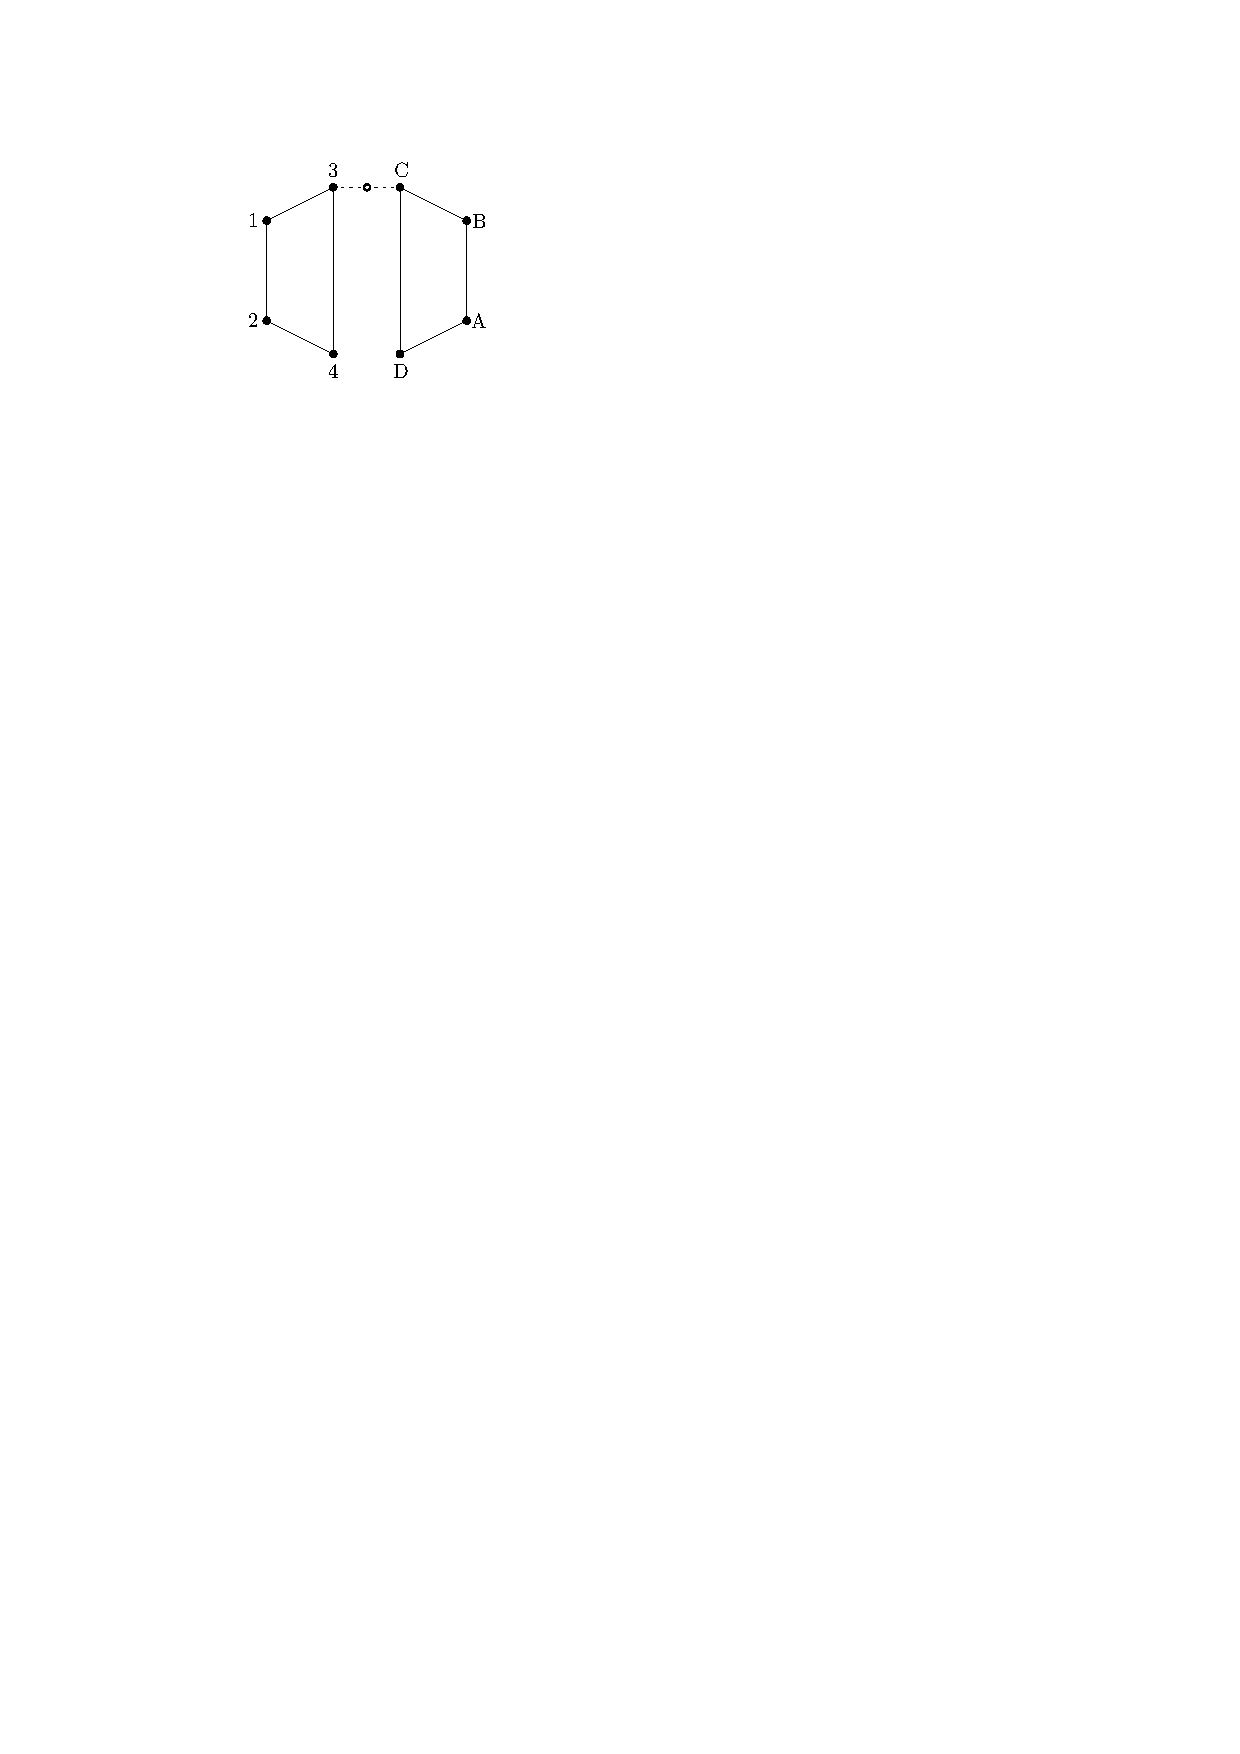
\includegraphics{img/bad-example-1} & 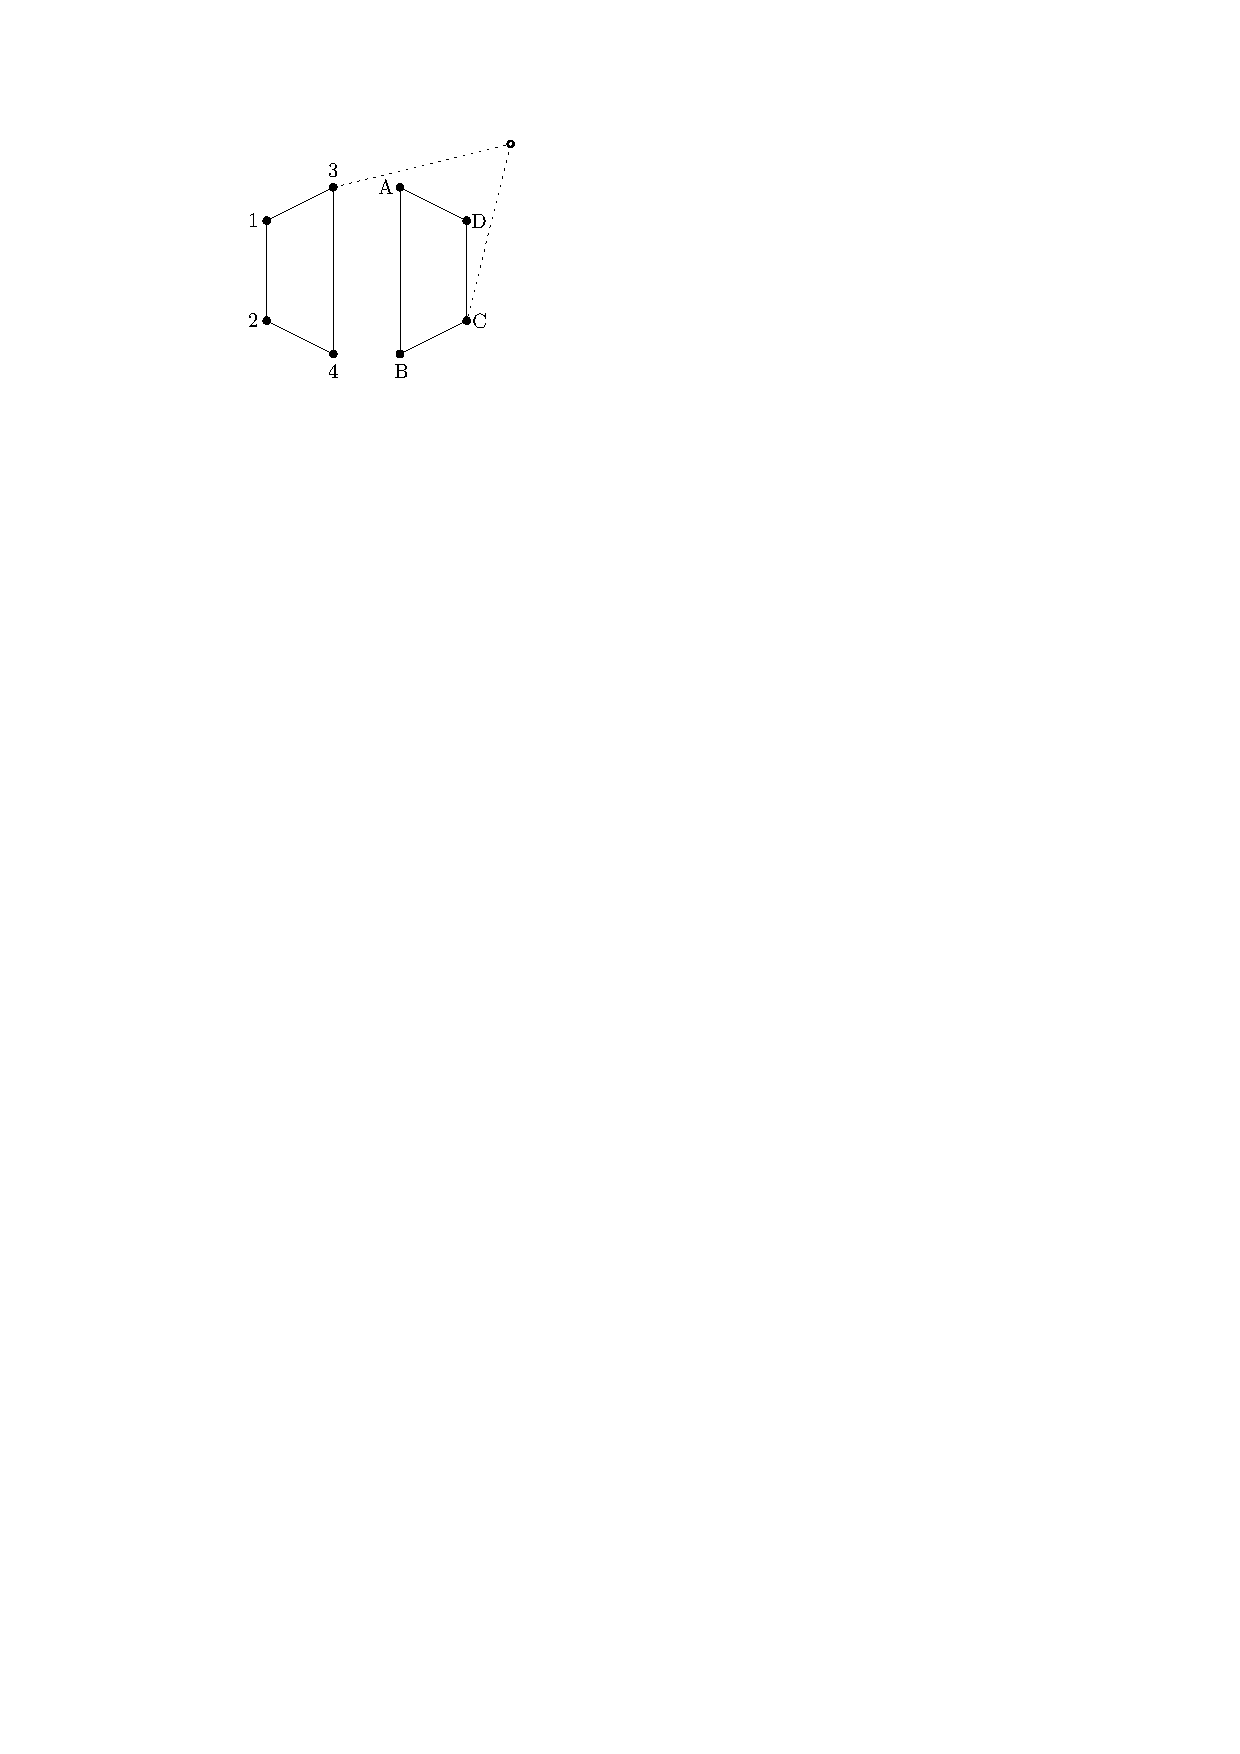
\includegraphics{img/bad-example-2}
    \end{tabular}
  }
  \caption{Two drawings of the same graph, $\mathcal{G}$, where making $\mathcal{G}$ connected requires the addition of both edges and vertices. In this case, $\mathcal G$ is made connected by adding the hollow vertex and two dashed edges.}
  \label{fig:bad-example}
\end{figure}

The motivation for this work comes from the problem of morphing
planar graph drawings, which has many applications \cite{erten.kobourov.ea:intersection,friedrich.eades:graph,gotsman.surazhsky:guaranteed,surazhsky.gotsman:controllable,surazhsky.gotsman:intrinsic} including
computer animation. Imagine an animator who wishes to animate a scene in which a character's expression
goes from neutral, to surprised, to happy. The animator can draw these
three faces, but does not want to hand-draw the 30--60 frames required
to animate the change of expression. This leads to the problem of computing a {\em morphing} (i.e., a continuous deformation) that transforms one drawing of a planar graph into
another drawing of the same planar graph while maintaining planarity
of the drawing throughout the deformation.
The morphing problem has been studied since 1944, when Cairns \cite{cairns:deformations}
showed that such a transformation always exists.  Since then, a sequence of results has shown
that such transformations can be done efficiently, so that the
vertex motion can be described concisely \cite{alamdari.angelini.ea:morphing,
angelini.dalozzo.ea:morphing,grunbaum.shephard:geometry,thomassen:deformations}.  The most recent such result
\cite{angelini.dalozzo.ea:morphing} shows that any planar drawing of
an $n$-vertex \emph{connected} planar graph can be morphed into any isomorphic
drawing using a sequence of $O(n)$ \emph{linear
morphs}, in which vertices move along linear trajectories at constant
speed.

The cited morphing algorithms require that the input graph, $\mathcal{G}$, be connected; however, in many applications this is not the case. Thus, before these morphing algorithms can be applied, $\mathcal{G}$ must be augmented to a connected graph, $\mathcal H$, and this augmentation must be compatible with all drawings of $\mathcal{G}$.  The complexity of the morph produced by a morphing algorithm depends on the size of $\mathcal H$.  Therefore, an augmentation with a small number of vertices is desirable. This motivates the theoretical question studied in the current paper.

%\paragraph{Formal Problem Statement and Main Result.} 
\subsection{Formal Problem Statement and Main Result} 

A \emph{drawing} of a labelled graph $\mathcal{G}=(V,E)$ is a one-to-one
function $\psi\colon V\to\R^2$.  A drawing is \emph{planar} if (a)~for
every pair of edges $uw$ and $xy$ in $E$, the open line segment with
endpoints $\psi(u)$ and $\psi(w)$ is disjoint from the open line
segment with endpoints $\psi(x)$ and $\psi(y)$ and (b)~for every edge
$uw$ and every vertex $y$, $\psi(y)$ is not contained in the open line
segment with endpoints $\psi(u)$ and $\psi(w)$.  Two planar drawings,
$\psi_1$ and $\psi_2$, of $\mathcal{G}$ are \emph{isomorphic} if
there exists a continuous family of planar drawings $\{\psi^{(t)}
\colon 0\le t\le 1\}$ of $\mathcal{G}$ such that $\psi^{(0)}=\psi_1$
and $\psi^{(1)}=\psi_2$.\footnote{By Cairn's result, this is equivalent
to saying that the two drawings of $G$ have the same rotation schemes,
the same cycle-vertex containment relationship, and the same outer face.}

Throughout this paper we will avoid repeatedly referencing drawing
functions like $\psi$.  Instead, we will talk about a labelled
graph $\mathcal{G}$ and $k$ isomorphic drawings $G_1,\ldots,G_k$ of
$\mathcal G$.  This means that each $G_i$ is the geometric graph given
by the drawing of $\mathcal{G}$ with some function $\psi_i$ and that
$\psi_1,\ldots,\psi_k$ are pairwise isomorphic. When necessary, we may talk
about the vertex $v$ in $G_i$ where $v$ is actually a (labelled) vertex
of $\mathcal{G}$; this should be taken to mean the vertex $\psi_i(v)$
in $G_i$.

We are now ready to state the main problem studied in this paper.  Given $k>1$
planar isomorphic drawings $G_1, \ldots, G_k$ of $\mathcal
G$, a \emph{compatible augmentation}, $\mathcal H$, of $\mathcal G$ is
a supergraph of $\mathcal G$ such that (1) $\mathcal H$ is connected
and (2) there exist planar isomorphic drawings, $H_1,
\ldots, H_k$, of $\mathcal H$ such that $H_i\supset G_i$ for every
$i\in\{1,\ldots,k\}$.  In this paper, we study the following extremal question: In the worst case
(over all $n$-vertex planar graphs, $\mathcal G$, and over all sets of
$k$ planar isomorphic drawings of $\mathcal{G}$), what is the size of the smallest compatible augmentation of $\mathcal G$?
In this paper, we show that, if $\mathcal{G}$
has $n$ vertices and $r$ connected components, there always exists a
compatible augmentation of size $O(nr^{1-1/k})$ and that this bound
is tight; there exists a graph $\mathcal G$
with $r$ components and $k$ drawings for which any compatible augmentation
has size $\Omega(nr^{1-1/k})$.  The upper bound holds for all $r\in\{2,\ldots,n\}$ and $k\ge 2$. The lower bound holds for all $r\in\{2,\ldots,n/3\}$ and $k\ge 2$.

These results show that the (worst-case) cost of an augmentation is very
sensitive to the number, $k$, of drawings, but only up to a point.
For a fixed value of $r$, our bounds range from $\Theta(nr^{1/2})$ (when
$k=2$) to $\Theta(nr)$ (for $k\ge \log r$).  On the other hand, for the
common case where $k=2$, our bounds vary from $\Theta(n)$ (when $r\in
O(1)$ up to $\Theta(n^{3/2})$ (when $r\in\Theta(n)$).  Neither $r$ nor $k$
causes the complexity of the augmentation to blow up beyond $\Theta(n^2)$.


\subsection{Related Work} 

To the best of our knowledge, there is little work on
compatible connectivity-augmentation of planar graphs, though
there is work on isomorphic triangulations of polygons.   In this setting, the goal is to compatibly triangulate the interior of two planar $n$-gons $P$ and $Q$.
%the graph $\mathcal{G}$ is a cycle and one has two planar straight-line drawings, $P$ and $Q$, of $\mathcal G$. The goal is to augment $\mathcal G$ (and the two drawings $P$ and $Q$) so that $\mathcal G$ becomes a near-triangulation, and $P$ and $Q$ become (geometric) triangulations of the interiors of the polygons whose boundaries are $P$ and $Q$.
Aronov \etal\ \cite{aronov.seidel.ea:compatible} showed that this can always
be accomplished with the addition of $O(n^2)$ vertices and that
$\Omega(n^2)$ vertices are sometimes necessary.  Kranakis and Urrutia
\cite{kranakis.urrutia:isomorphic} showed that the
number of triangles required is $O(n+pq)$ where $p$ and $q$ are the
number of reflex vertices of $P$ and $Q$, respectively.


Babikov \etal\ \cite{babikov.souvaine.ea:constructing} extended the result of Aronov \etal\ to polygons with holes. This work is the most closely related to ours because it encounters (the special case $k=2$ of) our problem as a subproblem. In their setting, $\mathcal G$ is a collection of $r$ cycles, and the two drawings are such that one cycle of $\mathcal G$ contains all the others in its interior and no other pair of cycles is nested. In the first stage of their algorithm, they build a connected supergraph $\mathcal{H}'$ of $\mathcal{G}$, but their supergraph has size $\Theta(n^2)$ in the worst case.  A byproduct of our main theorem is that this step of their algorithm could be done with a graph $\mathcal{H}'$ having only $O(nr^{1/2})$ edges (but completing this graph to a triangulation may still require $\Omega(n^2)$ edges in the worst case).

Finally, several papers~\cite{aghtu-acgg-08,rw-acpgg-12,t-capsg-12} have dealt with the problem of augmenting the connectivity of any (single) geometric planar graph while adding few vertices and edges.

\subsection{Outline} 

To guide the reader, we give a sketch of our upper bound proof: For each component, $\mathcal C_i$, of $\mathcal G$ we select a distinguished \emph{corner}, $a_i$, in $G_1$ (a corner is the space between two consecutive edges incident to some vertex of the outer face) and call it the \emph{attachment corner} for $\mathcal C_i$.  Notice that, since $G_1,\ldots,G_k$ are isomorphic, $a_i$ appears as a corner in each of $G_1,\ldots,G_k$. Next, for each $j\in \{1,\dots,k\}$, we define a connected geometric planar graph, $G_j^*$, obtained from $G_j$ after the addition of $r-1$ edges; these edges are not, in general, edges that take part in the final augmentation of $G_1,\ldots,G_k$ (in fact the edges of $G_j^*$ not in $G_j$ might be different from the edges of  $G_h^*$ not in $G_h$, if $j\neq h$). We traverse the boundary of the outer face
of $G_j^*$ to obtain a polygonal path, $\varphi_j$, of length $O(n)$ that comes
close to every corner of $G_j$.  The path $\varphi_j$ is then used to define an
integer distance $d_j(a_\ell,a_m)$ for any two corners $a_\ell$ and $a_m$. This distance includes information about the number of edges of $\varphi_j$ between $a_\ell$ and $a_m$ as well the sizes of some of the components visited while walking from $a_\ell$ to $a_m$ along $\varphi_j$.

Next, we take a leap into $k$ dimensions by using the distance
functions $d_1,\ldots,d_k$ to produce a $k$-dimensional point set
$X=\{x_1,\ldots,x_r\}$ that is contained in a hypercube of side-length $O(n)$.
This mapping has the property that, by adding a path of length $O(\|x_\ell
x_m\|)$ to $\mathcal G$, the corners $a_\ell$ and $a_m$ can be joined
in each of $G_1,\ldots,G_k$ while preserving planarity.
Now, since the point set $X$ is in $\R^k$, has $r$ points, and
is contained in a hypercube of side-length $O(n)$, a classic
result on the Travelling Salesman Problem \cite{few:shortest,moran:on} implies that it has a spanning path whose length, measured in the $\ell_\infty$ norm,
is $O(nr^{1-1/k})$.\footnote{The original argument was for the standard
$\ell_2$ norm and has an extra $\sqrt{k}$ factor.  This factor disappears
in the $\ell_\infty$ norm.}  This implies that $\mathcal G$ can be made
connected with a collection of $r-1$ paths, whose endpoints are the
corners $a_1,\ldots,a_r$, having total size $O(nr^{1-1/k})$, and
that each of these paths can be drawn in a planar fashion in each
of $G_1,\ldots,G_k$.
At this point, it remains to show that these $r-1$ paths
can each be drawn in each of $G_1,\ldots,G_k$ without crossing
each other.  This part of the proof involves carefully winding these
paths around the components in $G_1,\ldots,G_k$ using paths close
to the paths $\varphi_1,\ldots,\varphi_k$ defined above.
%This part of the proof resembles the first part of the proof of Babikov \etal\ \cite{babikov.souvaine.ea:constructing}, but is complicated by the fact that we have to be quite careful that the number of edges in these paths remains in $O(nr^{1-1/k})$.

The lower bound involves a sequence of paths whose vertices correspond to the vertices of
a nested set of regular $\lfloor n/r\rfloor$-gons.

The remainder of the paper is organized as follows: In
Section~\ref{section:Trivial components} we solve the special case in which $\mathcal G$ has no edges. This
case is already non-trivial and introduces some of the
main ideas used in solving the full problem, which is tackled in
Section~\ref{section:General}. Section~\ref{section:Lower bound}
proves the lower bound. Due to space constraints, some of the proofs are only included in the full version of the paper, which is attached as an Appendix.
%The paper concludes with
%Section~\ref{section:Conclusions}, which summarizes and presents
%directions for future research.


%%%%%%%%%
\section{Upper bounds for trivial components}\label{section:Trivial components}
As a warmup, we consider a (trivial) graph containing $n$ vertices and no edges.
Before constructing a compatible augmentation, we provide a subroutine
that constructs a ``short'' planar spanning path of a given ordered set  of points.

\subsection{Spanning paths of point sets}
Let $S$ be a set of $n$ points in the plane with distinct $x$-coordinates.
Given a point $v\in S$, let $\rank(v)$ denote the number of points of $S$ having smaller $x$-coordinate than $v$.
Given an arbitrary order $(v_1, v_2, \ldots, v_n)$ of the points of $S$, we show how to construct a planar path that connects them in this order and such that the number of vertices between $v_{i-1}$ and $v_{i}$ is $O(|\rank(v_i) - \rank(v_{i-1})|)$, for each $i\in \{2, \dots, n\}$.

%want to construct a path $R$ that connects them in this order  such that $$|R|  = O\left(\sum_{i=1}^{n-1} |\rank(v_i) - \rank(v_{i+1})| \right)\ .$$
This paper uses the $|\cdot|$ operator in several ways.  Namely, for a real number, $x$, we denote by $|x|$ the absolute value of $x$; for a walk, $R$, we denote by $|R|$ the number of edges traversed by $R$; also, for a (weakly) simple polygon, $P$, we denote by $|P|$ the number of edges of~$P$.

Consider a horizontal line $\ell$ below $S$ and let $\pi$ be the closed halfspace supported by $\ell$ that contains $S$.  We present an algorithm that constructs $R$ iteratively; during the $i$th iteration of the algorithm, the path is extended with $O(|\rank(v_i) - \rank(v_{i-1})|)$ vertices to include $v_i$.  For each $i\in \{1,\dots,n\}$, after the $i$th iteration of the algorithm, we maintain the invariant that $\ell$ does not intersect $R$, and we also maintain the \emph{escape invariant} which is defined as follows:
For each $j\in \{i, \dots, n\}$, there is a closed cone $\Delta_{j}$ with apex $u_{j}$ such that (1) $u_j$ lies above $v_j$ and has the same $x$-coordinate as $v_j$ ($u_j =v_j$ if $j = i$), (2) $\Delta_j$ contains $v_j$ and no other point of $S$, (3) $\Delta_j$ contains the ray originating at $v_j$ in the direction of the negative $y$-axis, (4) $\Delta_j$ does not intersect $R$, and (5) $\Delta_h$ and $\Delta_j$ are disjoint inside $\pi$, for every $h\in \{i,\dots,n\}$ with $h\neq j$.

%(2) $\Delta_j$ contains the ray originating at $v_j$ in the direction of the negative $y$-axis, (3) $\Delta_{i}$ does not intersect $R$, except at $v_{i}$; also, for every $j\in \{i+1,\dots,n\}$, there is a cone $\Delta_j$ with apex $u_j$ such that (1) $u_j$ lies above $v_j$ and has the same $x$-coordinate as $v_j$, (2) $\Delta_j$ contains $v_j$ and no other point of $S$, (3) $\Delta_j$ contains the ray originating at $v_j$ in the direction of the negative $y$-axis, (4) $\Delta_j$ does not intersect $R$, and (5) $\Delta_h$ and $\Delta_j$ are disjoint inside $\pi$, for every $h\in \{i,\dots,n\}$ with $h\neq j$.
%To construct $R$, we add the points of $S$, one by one according to the given order, while maintaining the escape invariant.

Initialize $R$ as a path that consists of the single vertex $v_1$. In order to establish the escape invariant, we define $u_1=v_1$; also, for each $j\in \{2,\dots,n\}$, we define $u_j$ as an arbitrary translation up of $v_j$; further, for each $j\in \{1,\dots,n\}$, we let $\Delta_j$ be a cone with apex on $u_j$ sufficiently narrow so that these cones do not intersect inside $\pi$; see Figure~\ref{fig:Dented Halfspace} (left).

Now assume that $R$ is a path connecting $v_1$ with $v_j$, for some $j\in \{1,\dots,n-1\}$. We extend $R$ by appending a
path that connects $v_j$ with $v_{j+1}$.

First, we translate $\Delta_{j+1}$ down until its apex $u_{j+1}$ coincides with $v_{j+1}$. Let $\pi_j$ be the closure of the set obtained from $\pi$ by removing $\Delta_h$, for every $h\in\{j,j+1,\ldots,n\}$; see Figure~\ref{fig:Dented Halfspace} (right). That is, $\pi_j$ is a halfspace with dents made by the removal of $n-j+1$ cones.
%Therefore, the number of segments on the boundary of $\pi_j$ is $O(n-j)$.
Observe that, for every pair of apexes $u_i$ and $u_h$, with $i,h\geq j$, the boundary of $\pi_j$
contains a path from $u_i$ to $u_h$ with $O(|\rank(v_i)-\rank(v_h)|)$ edges.
Because $\ell$ does not intersect $R$ and by the escape invariant, the boundary of $\pi_j$ intersects $R$ only at $v_j$. Moreover, again by the escape invariant, for each $v_i$ with $i > j$, $v_i$ lies outside of~$\pi_j$ except for $v_{j+1}$ that lies on its boundary. Because both $v_j$ and $v_{j+1}$ lie on the boundary of $\pi_j$, which does not intersect $R$ other than at $v_j$, we can connect $v_j$ with $v_{j+1}$ via a path contained in the boundary of~$\pi_j$ with length $O(|\rank(v_j) - \rank(v_{j+1})|)$. In this way, we extend $R$ to a planar path that connects $v_1$ with $v_{j+1}$.

\begin{figure}[tb]
\centering
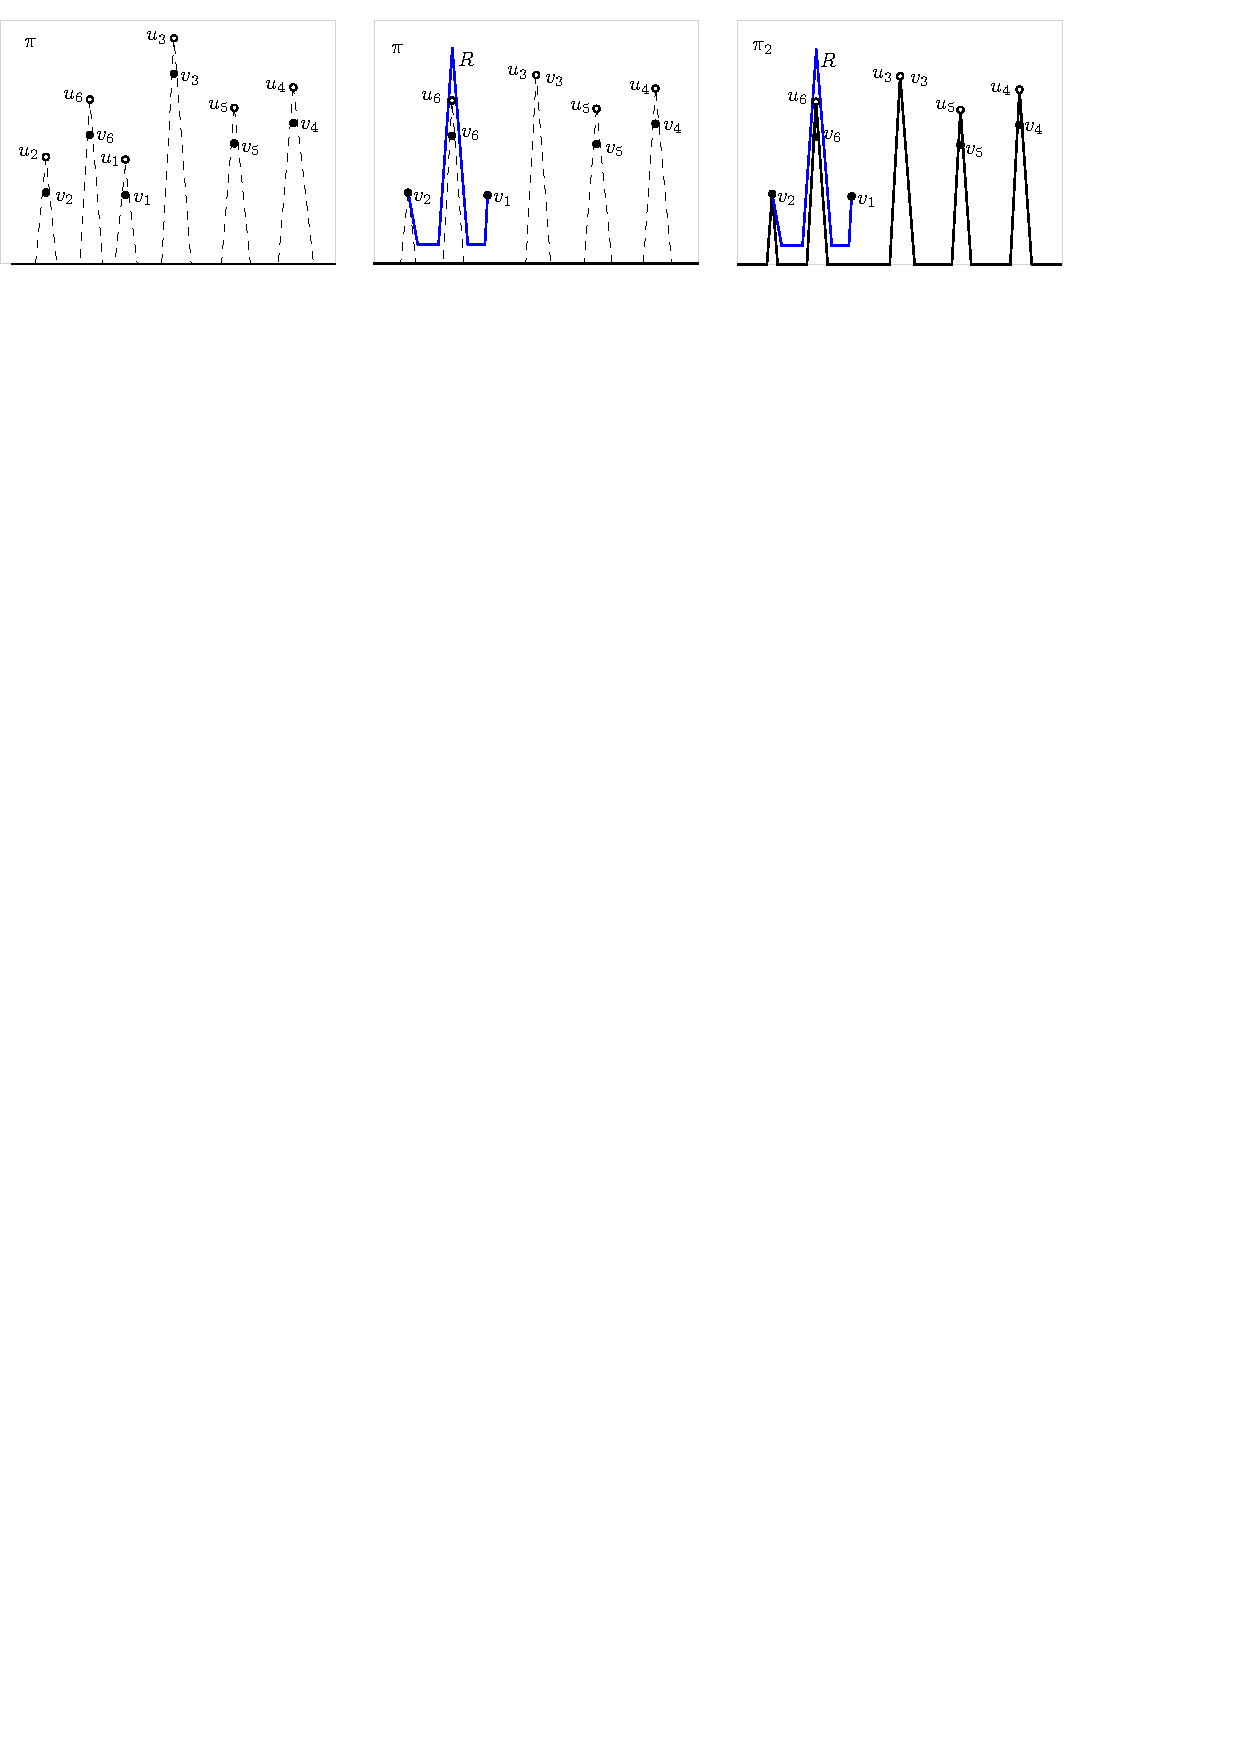
\includegraphics[width=.98\textwidth]{img/DentedHalfspace.pdf}
\caption{\small The halfplane $\pi$ and the cones $\Delta_1,\ldots,\Delta_n$ with apexes at $u_1,\ldots,u_n$ (left);
the halfspace $\pi$ before the removal of $n-j+1$ cones (middle); and the boundary of $\pi_2$ containing a path from $v_2$ to $v_3$  (right).}
\label{fig:Dented Halfspace}
\end{figure}


After connecting $v_j$ with $v_{j+1}$, for each $h\in\{j{+}2,\ldots,n\}$, either $\Delta_h$ is disjoint from $R$, or it shares some portion of its boundary with $R$. However, the interior of $\Delta_h$ does not intersect $R$.
To preserve the escape invariant, for each $h\in\{j{+}2,\ldots,n\}$, we translate $\pi$ and $\Delta_h$ downwards by a sufficiently small amount, $\varepsilon$, and we scale $\Delta_{j+1}$ horizontally down, while keeping its apex at $v_{j+1}$. To conclude, each translated or scaled cone is contained in the previous one, $u_h$ lies above $v_h$, for each $h\in\{j+2,\ldots,n\}$, and $u_{j+1}$ coincides with $v_{j+1}$. Therefore, by choosing $\varepsilon$ sufficiently small, we maintain the escape invariant and obtain the following result.

\begin{lemma}\label{lemma:Compatible augmentation for trivial components} \appendixproof
Given an order $(v_1, \ldots, v_n)$ of the vertices of $S$, there exists a planar path $R$ that connects every point of $S$ in the given order such that the number of vertices of $R$ between $v_{i-1}$ and $v_{i}$ is $O(|\rank(v_i) - \rank(v_{i-1})|)$, for each $i\in \{2,\dots,n\}$.
\end{lemma}

%\vspace{-.1in}
\subsection{Compatible drawings of point sets}%\vspace{-.1in}
Recall that in this section $\mathcal G$ is a graph with $n$ trivial components.
Let $G_1, \ldots, G_k$ be $k>1$ isomorphic drawings of $\mathcal G$, i.e., $G_i$ is a sequence of $n$ points in the plane.
Assume without loss of generality that no two points of $G_i$ share the same $x$-coordinate.
Given a vertex $v$ of $\mathcal G$, let $\rank_{G_i}(v)$ denote the number of points of $G_i$ having smaller $x$-coordinate than $v$, and let $x_v = (\rank_{G_1}(v), \ldots, \rank_{G_k}(v))$ be a point in the integer grid $[0;n-1]^k$ in $\mathbb{R}^k$.  Let $X = \{x_v : v\in V(\mathcal G)\}$ and let $P$ be the shortest Hamiltonian path of $X$ using the $\ell_\infty$ norm.  It is known that the length of
$P$ is $O(n^{2-1/k})$~\cite{few:shortest,moran:on}.
Note that the order of the points of $P$ induces an order on the vertices of $\mathcal G$ and hence, an order on the vertices of each $G_i$.


\begin{theorem}\label{theorem:points}
For each $i\in \{1,\dots,n\}$, we can construct a path $R_i$ of length $O(n^{2-1/k})$ that connects every point of $G_i$ so that $G_i\cup R_i$ is planar. Moreover, for any distinct $i,j\in \{1,\dots,n\}$, $G_i\cup R_i$ and $G_j\cup R_j$ are~isomorphic.
\end{theorem}
%\vspace{-.2in}
\begin{proof}
By relabelling, let $(v_1, \ldots, v_n)$ denote the order of the vertices of $\mathcal{G}$ induced by $P$.  The augmented graph $\mathcal{H}$ is a path that visits the vertices $v_1,\ldots,v_n$ in this order. Letting $d_j$ denote the $\ell_\infty$ distance between $x_{v_j}$ and $x_{v_{j+1}}$, the path $\mathcal{H}$ includes an additional $O(d_j)$ vertices between $v_{j}$ and $v_{j+1}$.  It follows that the number of vertices
in $\mathcal{H}$ is proportional to the length of $P$, which is $O(n^{2-1/k})$.

For each $G_i$, we use Lemma~\ref{lemma:Compatible augmentation for trivial components} to draw $\mathcal{H}$ as a planar path, $R_i$,
that connects the vertices $v_1,\ldots,v_n$ in this order in the drawing $G_i$.
Since $d_j\ge |\rank_{G_i}(v_j) - \rank_{G_i}(v_{j+1})|$, the $O(d_j)$
vertices in $\mathcal{H}$ between $v_j$ and $v_{j+1}$ are enough to
draw the $O(|\rank_{G_i}(v_j) - \rank_{G_i}(v_{j+1})|)$ vertices in $R_i$
between $v_j$ and $v_{j+1}$.
Since the vertices of each $G_i$ are connected in the same order,
$G_i\cup R_i$ is isomorphic to $G_j\cup R_j$ for each $i,j\in\{1,\ldots,k\}$.
\end{proof}


\section{The general problem}\label{section:General}
In this section, we extend the result presented in
Section~\ref{section:Trivial components} to graphs with
non-trivial components.  We follow the same general scheme used in
Section~\ref{section:Trivial components} for the case of trivial
(isolated vertex) components:  We define $k$ different
orderings of the components of $\mathcal G$ and use these orderings (and
the sizes of these components) to define an $r$-point set, $X$, in $\R^k$. A
short path that visits all points in $X$ is then translated back into
a short path, $R$, that visits all components of $\mathcal G$. The path
$R$ is then
added, as a polygonal path, $R_i$, to each drawing, $G_i$, of $\mathcal G$.

Unlike the case in which
components are isolated vertices, there is no natural ordering of the
components of $G_i$, so we must define one. Also, the drawing
of path $R_i$ is considerably more complicated.  In Section~\ref{section:Trivial components}, $R_i$ is drawn incrementally, and always passes above components that are not yet included in $R_i$ and below components that are already included in $R_i$.  In this section, we redefine ``above'' and ``below''. The cost of going above or below a component depends on its size and structure.
%We begin with some careful definitions because, when a component is not an isolated vertex, we have to be considerably more specific about how the path, $R$, visits it.


\subsection{Preliminaries}\label{section:Preliminaries}
Let $C$ be a connected geometric planar graph. Let $v_0, v_1, \ldots, v_k, v_0$ be the sequence of vertices of $C$ visited by a counterclockwise
Eulerian tour along the boundary of the outer face of $C$. Note that
$v_i$ may be equal to $v_j$ for some $i\neq j$.  A vertex $v_i$
in this sequence is called a \emph{corner} of $C$.  We consider the boundary of $C$, denoted by $\partial C$, to be the
boundary of the weakly-simple polygon $(v_0, \ldots, v_k, v_0)$ whose
vertex set is the set of corners of $C$.\footnote{More formally, $\partial C$ is the boundary of the unbounded component of $\mathbb{R}^2\setminus C$, where we treat $C$ as the union of all its edges and vertices.}

Let $\varepsilon >0$. For each corner $v_i$ of $\partial C$, let $\ell_i$ be the half-line starting at $v_i$ that bisects the angle between the edges $v_{i-1}v_i$ and $v_i v_{i+1}$ in the outer face of $C$. Let $z_i$ be the point at distance $\varepsilon$ from $v_i$ along $\ell_i$. We call $z_i$ the \emph{$\varepsilon$-copy} of $v_i$. Let $\partial_\varepsilon C$ be the polygon defined by the sequence $(z_0, z_1, \ldots, z_k, z_0)$, i.e., $\partial_\varepsilon C$ is isomorphic to $\partial C$ (but not necessarily to $C$). We call $\partial_\varepsilon C$ the \emph{$\varepsilon$-fattening} of $C$.
An $\varepsilon$-fattening $\partial_\varepsilon C$ is \emph{simple} if $\partial_\varepsilon C$  is a simple polygon that contains~$C$.
Note that $\partial_\varepsilon C$ is simple, provided that $\varepsilon$ is sufficiently small. In this paper, we consider only simple $\varepsilon$-fattenings; see Figure~\ref{fig:Blowing}. Note that the (graph) distance between two corners of $\partial C$ along the boundary of $C$ is the same as the distance between their $\varepsilon$-copies along~$\partial_\varepsilon C$.

%%%%%%%%%%%%%%%
\subsection{Connected augmentations}\label{section: connected augmentations}
Let $G$ be a geometric planar graph with $r$ connected components such that each component is adjacent to the outer face.
Two vertices are {\em visible} if the open segment joining them does not intersect $G$.
Let $T_G$ be a smallest set of edges of the visibility graph of $G$ that need to be added to $G$ to make it connected.
As there are always two components containing mutually visible vertices, we can connect them and repeat recursively.  Thus, $T_G$ has $r-1$ edges. (Loosely, we can think of $T_G$ as a spanning tree of $G$'s components.) Let $G^* = G\cup T_G$.  We say that $G^*$ is a \emph{connected augmentation} of $G$; see Figure~\ref{fig:Blowing}.

\begin{figure}[h]
\centering
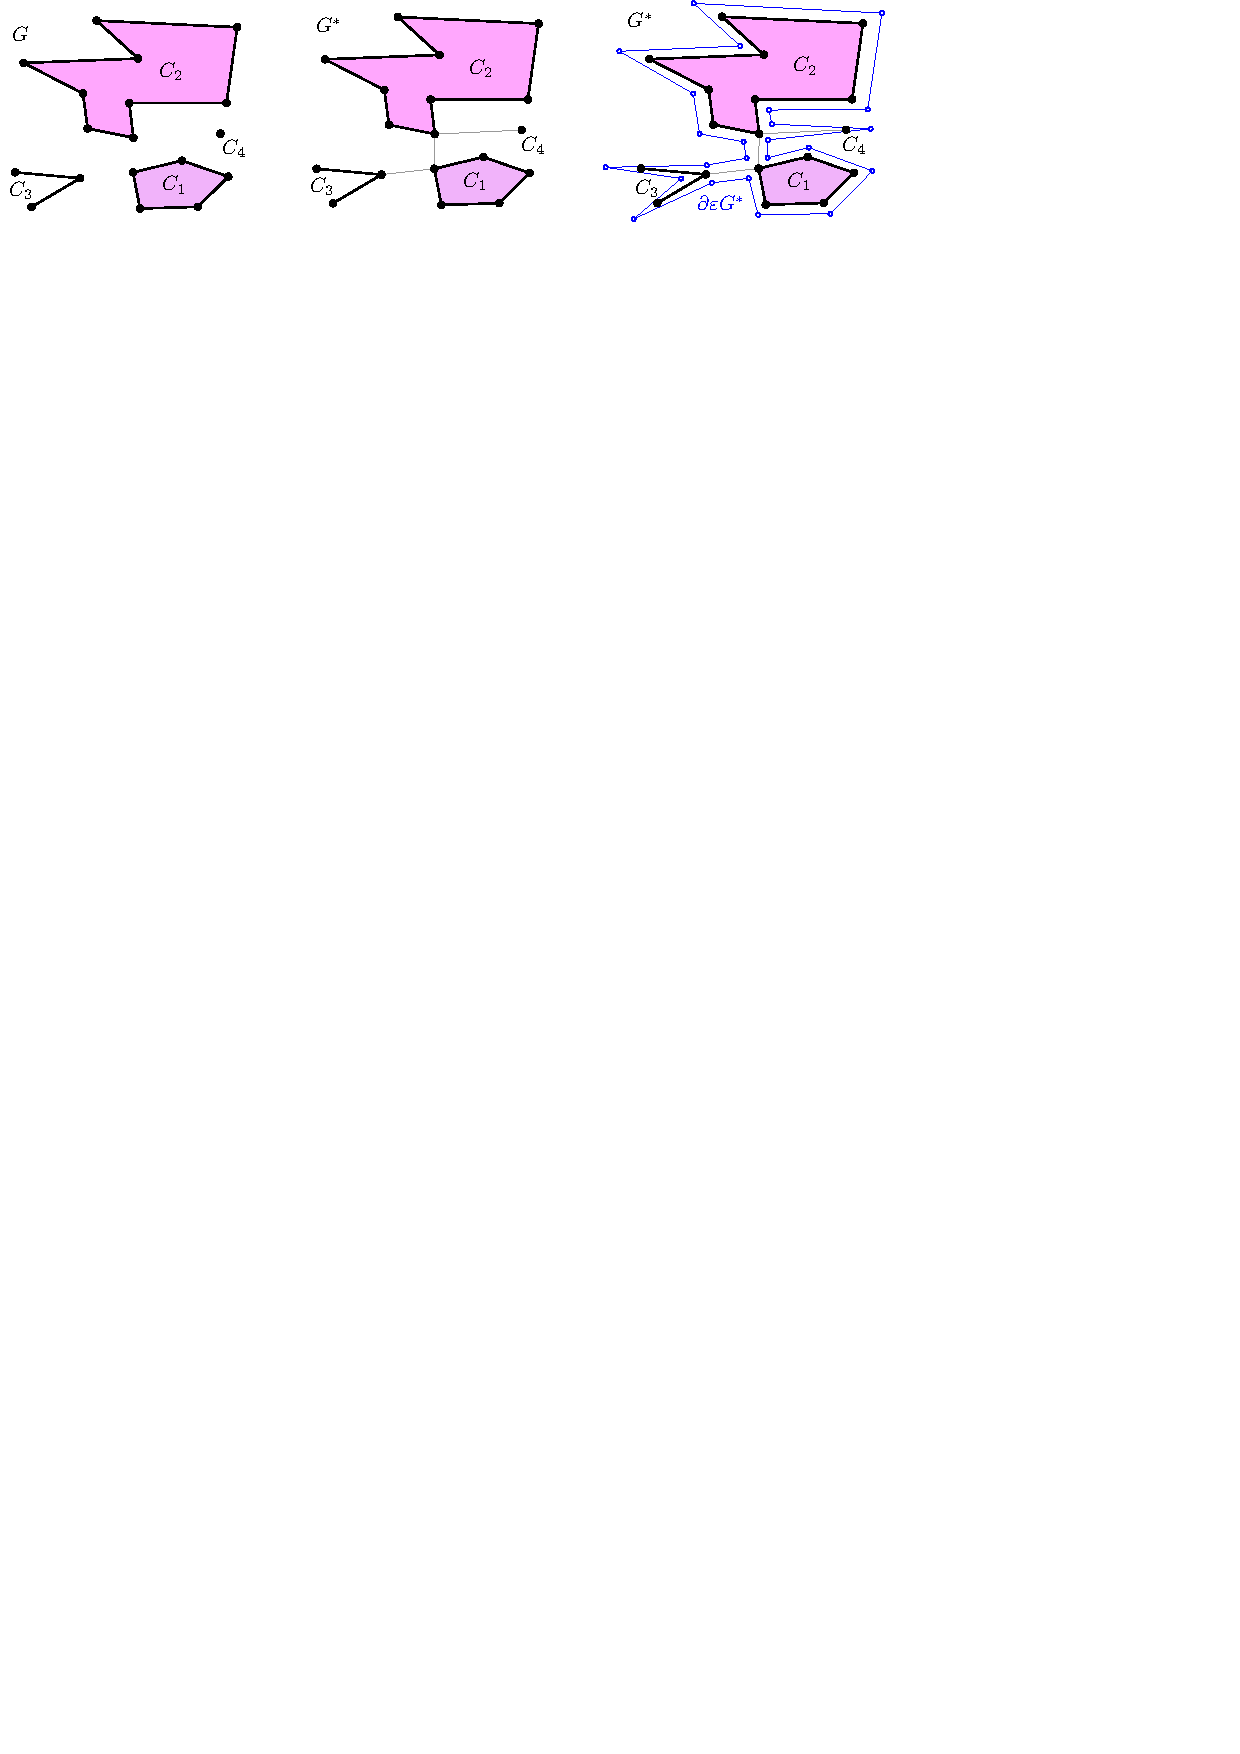
\includegraphics{img/Blowing.pdf}
%[width=1\textwidth]
\caption{\small A geometric graph $G$ (left); a connected augmentation, $G^*$, of $G$ (middle); and the $\varepsilon$-fattening, $\partial_\varepsilon G^*$ (right).}
\label{fig:Blowing}
\end{figure}

Let $C_1, \ldots, C_r$ be the components of $G$.
%Recall that we consider $\partial C_i$ to be the boundary of a weakly-simple polygon. Therefore, even though a vertex of $C_i$ can appear multiple times along $\partial C_i$, we consider them as different corners of $\partial C_i$.
For each $i\in \{1,\dots,r\}$, let $a_i\in C_i$ be an arbitrary corner of $\partial C_i$ (note that $a_i$ is adjacent to the outer face).
We call $a_i$ the \emph{attachment corner} of $C_i$.

Let $\varphi$ be the path on the corners of $\partial G^*$ (hence $\varphi$ is also a walk on the vertices of $\partial G^*$) obtained by splitting $\partial G^*$ at the corner $a_1$. That is, $\varphi$ is a path that visits every corner of $\partial G^*$ exactly once except for $a_1$, that is visited twice.
Given two corners $u$ and $v$ in $\partial G^*$, let $\varphi(u,v)$ denote
the unique path in $\varphi$ that connects $u$ with $v$. Let $A(u,v)$ be
the set of attachment corners of $G$ visited by $\varphi(u,v)$. Define
    $ \sigma_G(u,v) = |\varphi(u,v)| + \sum_{a_i\in A(u,v)}|\partial C_i|$,
which we call the \emph{cost} of going from $u$ to $v$. 
%Intuitively, the cost of going from $u$ to $v$ depends heavily on the number of corners visited by $\varphi(u,v)$.

\begin{lemma}\label{lemma:Contained in integer grid}\appendixproof
  If $a$ is an attachment corner of $G$, then $\sigma_G(a_1, a) < 4n$. Moreover, if $b$ is another attachment corner of $G$, then
  $\sigma_G(a, b) =  |\sigma_G(a_1, a)- \sigma_G(a_1, b)|$.
\end{lemma}
%\vspace{-.1in}
\subsection{Spanning paths for connected augmentations}\label{section:Spanning paths for connected augmentations}
Let $a_1, \ldots, a_r$ be an arbitrary order of the attachment corners of $G$ (we can get the incremental indexing by relabeling the components).
Consider a planar path $R = (\rho_1, \rho_2, \ldots, \rho_t)$ that passes through all attachment corners of $G$ and through no other vertices of $G$ ($R$ may have vertices not in $G$). We say that $C_i$ {\em lies to the right of $R$} if, for each $j\in\{1,\ldots,t\}$ such that $\rho_j=a_i$ is an attachment corner of $G$, $\rho_{j-1}$ and $\rho_{j+1}$ appear as consecutive vertices when sorting the neighbors of $a_i$ in clockwise order around $a_i$ in the graph $G\cup R$; see Figure~\ref{fig:Neighborhood} (left).

We want $R$ to connect the attachment corners of $G$ in the given order, i.e., if $i < j$, then $a_i$ is visited before $a_j$ by $R$. We want to construct $R$ so that each component $C_i$ of $G$ lies to the right of~$R$.
Moreover, we want the subpath of $R$ between $a_j$ and $a_{j+1}$ to have $O(\sigma_G(a_j, a_{j+1}))$ vertices. 
We initialize $R$ with the trivial path that contains only $a_1$, and then modify $R$ iteratively, so that each new corner $a_i$ is included in $R$.
Recall that  for any given $\varepsilon >0$, $\partial_\varepsilon G^*$ denotes the $\varepsilon$-fattening of $G^*$ (see Section~\ref{section:Preliminaries}).
Let $\mu>0$ be a small constant to be specified later.
Initially, let $\varepsilon = 2\mu$ and let $\delta = \mu/2$. Let $\lambda < \mu/2^{r+1}$ be a constant sufficiently small so that $\partial_\lambda C_i \cap \partial_\lambda C_j = \emptyset$ for any distinct $i,j\in\{1,\ldots,r\}$.
Throughout, $\lambda$ remains constant while $\varepsilon$ and $\delta$ are redefined at each iteration. However, as an invariant we maintain $\lambda < \delta < \varepsilon$.

\begin{figure}[h!]
\centering
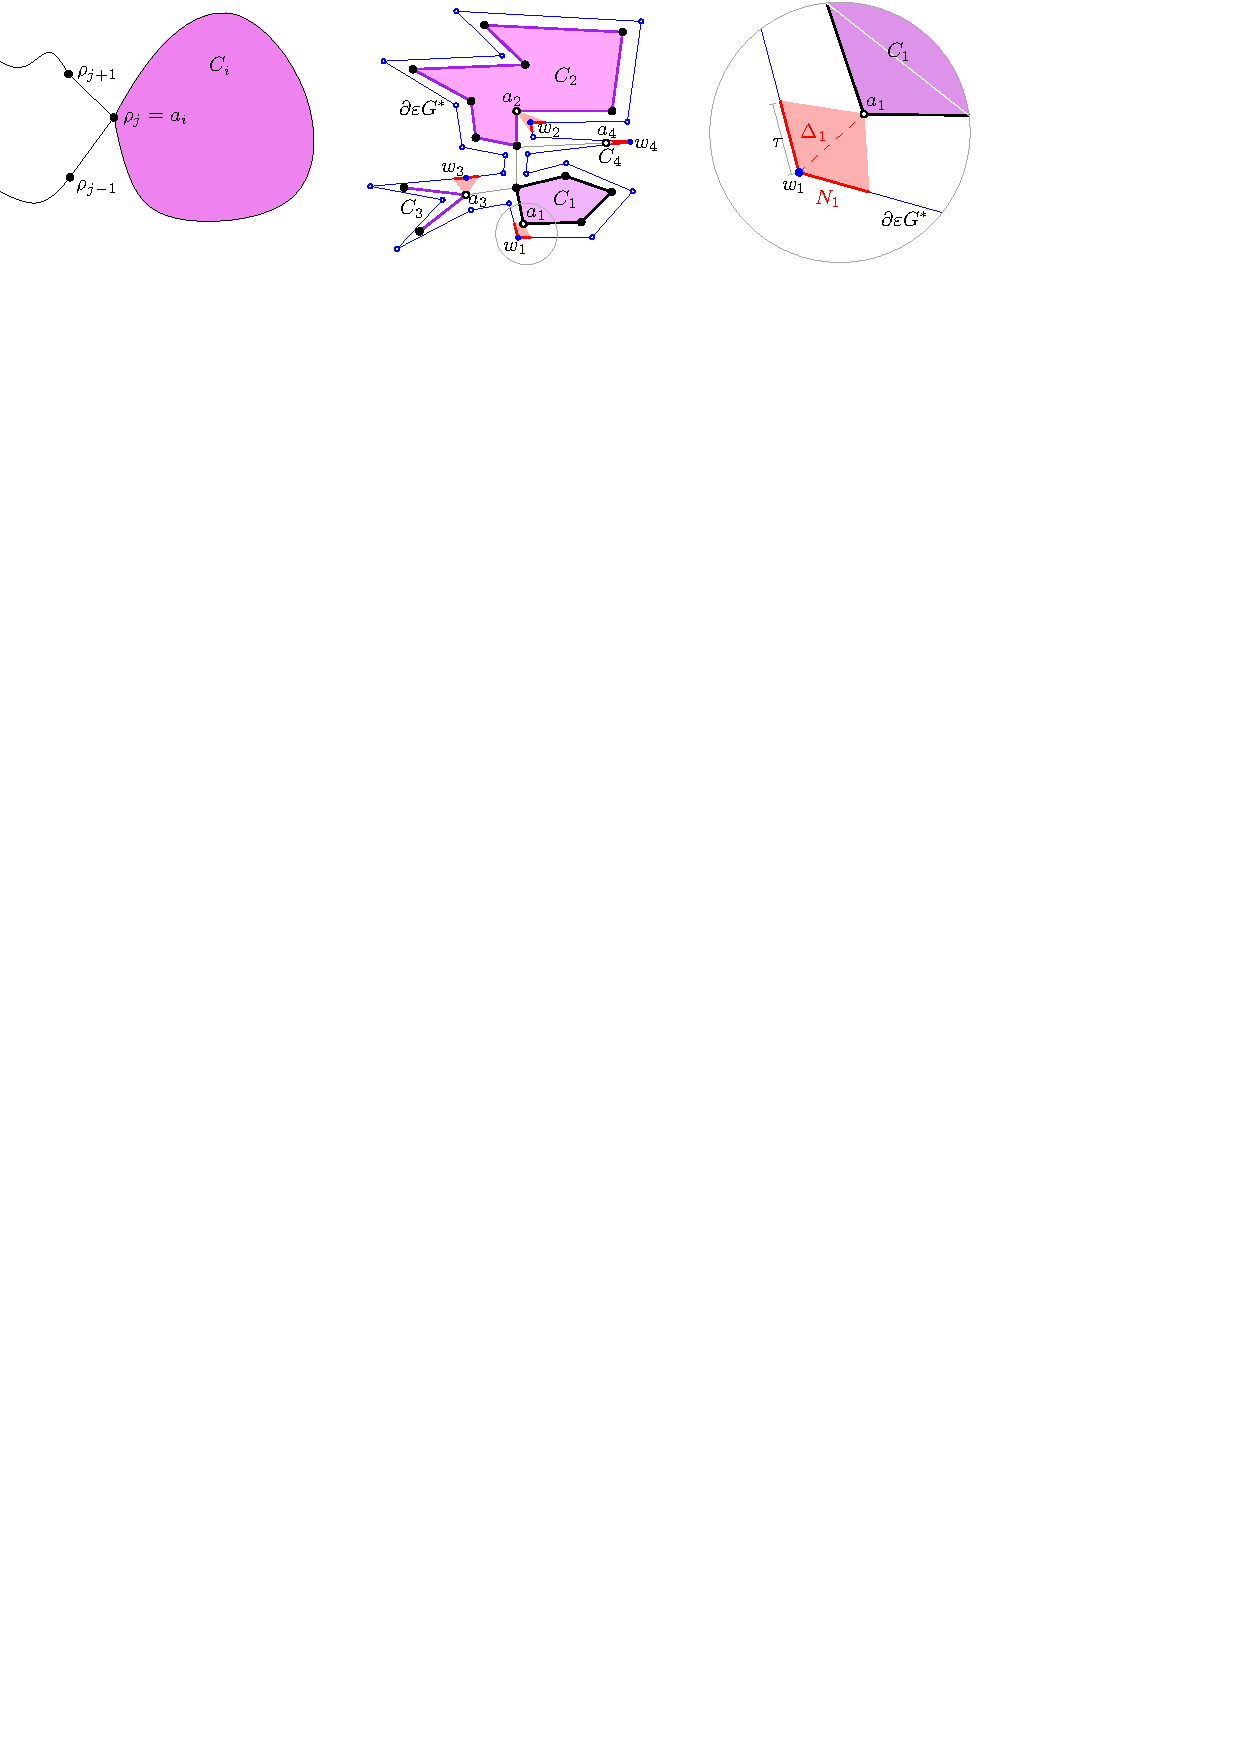
\includegraphics[width=1\textwidth]{img/Neighborhood.pdf}
\caption{\small The component $C_i$ is to the right of the path $R=(\rho_1,\ldots,\rho_t)$ (left); the $\epsilon$-fattening of $G^*$ and the ``cones'' $\Delta_1,\ldots,\Delta_r$ (middle); and a close look at the ``cone'' $\Delta_1$ (right).}
\label{fig:Neighborhood}
\end{figure}

For each $i\in \{1,\dots,r\}$, let $w_i$ be the $\varepsilon$-copy of  $a_i$.
Split $\partial_\varepsilon G^*$ at $w_1$, i.e., $\partial_\varepsilon G^*$ is a path with both endpoints equal to $w_1$.
By choosing $\varepsilon$ sufficiently small, we guarantee that $\partial_\varepsilon G^*$ is simple, i.e., $\partial_\varepsilon G^*$ is isomorphic to $\varphi$.
We say that two points in the plane are \emph{$R$-visible} if the open segment joining them does not intersect $R$.
Let $\tau >0$. For each $i\in \{1,\dots,r\}$ such that $a_i$ is not an interior point of $R$, consider the set of points $N_i\subset \partial_\varepsilon G^*$ that are at distance at most $\tau$ from $w_i$.
Let $\Delta_i$ be the convex hull of $N_i\cup \{a_i\}$, i.e., $\Delta_i$ is a ``cone'' with apex at $a_i$; see Figure~\ref{fig:Neighborhood} (middle, right). We deliberately misuse the word ``cone'' here because the ``cones'' $\Delta_1,\ldots,\Delta_r$ in this section play the same roles as the cones $\Delta_1,\ldots,\Delta_n$ in Section~\ref{section:Trivial components}.

While constructing $R$, we also maintain the \emph{escape invariant} which is defined as follows. Assume that $R$ so far connects $a_1$ with $a_i$, for some $i\in \{1,\dots,r-1\}$. Then: (1) $R$ intersects neither $\partial_\varepsilon G^*$ nor its unbounded face; (2) for each $j>i$, $R$ intersects neither the simple polygon bounded by $\partial_\delta C_j$ nor the cone $\Delta_j$; and (3) $\Delta_h\cap \Delta_j = \emptyset$, for any distinct $h,j\in\{1,\ldots,r\}$. In particular, the escape invariant implies that every point in $N_j$ (including $w_j$) is $R$-visible from $a_j$. The escape invariant holds when $R=\{a_1\}$, provided that $\tau$ is sufficiently small.


Assume that we have constructed a path $R$ that connects $a_1$ with $a_j$, for some $j\in\{1,\ldots,r-1\}$, and that the escape invariant holds.  To extend $R$, we create a new path that connects $a_j$ with $a_{j+1}$ without crossing $R$ while maintaining the escape invariant.  Recall that we consider $\partial_\varepsilon G^*$ to be a path with both endpoints on~$w_1$.

The first part of the path connecting $a_j$ with $a_{j+1}$ consists of a path connecting $a_j$ with $w_j$. If $j=1$, or if $j>1$ and $R$ together with the edge $a_j w_j$ leaves $C_j$ to its right, then connect $a_j$ with $w_j$ via a straight-line segment; since $w_j$ is $R$-visible from $a_j$, this segment does not cross $R$. Otherwise, connect $a_j$ with $\partial_\lambda C_j$ via a straight-line segment and traverse $\partial_\lambda C_j$ in clockwise order without crossing $R$ before moving to $w_j$ on $\partial_\varepsilon G^*$. In this way, we guarantee that $C_j$ lies to the right of the constructed path; see Figure~\ref{fig: Component to the right} for an illustration. Because $\lambda < \delta < \varepsilon$ and since $a_i\in V(R)$, the escape invariant is preserved.


%If $j>1$, then we need to be careful in the neighbourhood of $a_j$ as we want $R$ to have $C_j$ to its right. If the path $R$ together with the edge $a_j w_j$ leaves $C_j$ to its right, then walk from $a_j$ to $w_j$ in straight line. Because the escape invariant holds, we know that $w_j$ is $R$-visible form $a_j$ and hence, this edge does not cross $R$. If $R$ together with $a_j w_j$ does not leave $C_j$ to its right, then walk from $a_j$ to $\partial_\lambda C_j$ instead and traverse $\partial_\lambda C_j$ in clockwise order without crossing $R$ before moving to $w_j$ on $\partial_\varepsilon G^*$. In this way, we guarantee that $C_j$ lies to the right of the constructed path; see Figure~\ref{fig: Component to the right} for an illustration. Because $\lambda < \delta < \varepsilon$ and since $a_i\in V(R)$, the escape invariant is preserved.

\begin{figure}[t]
\centering
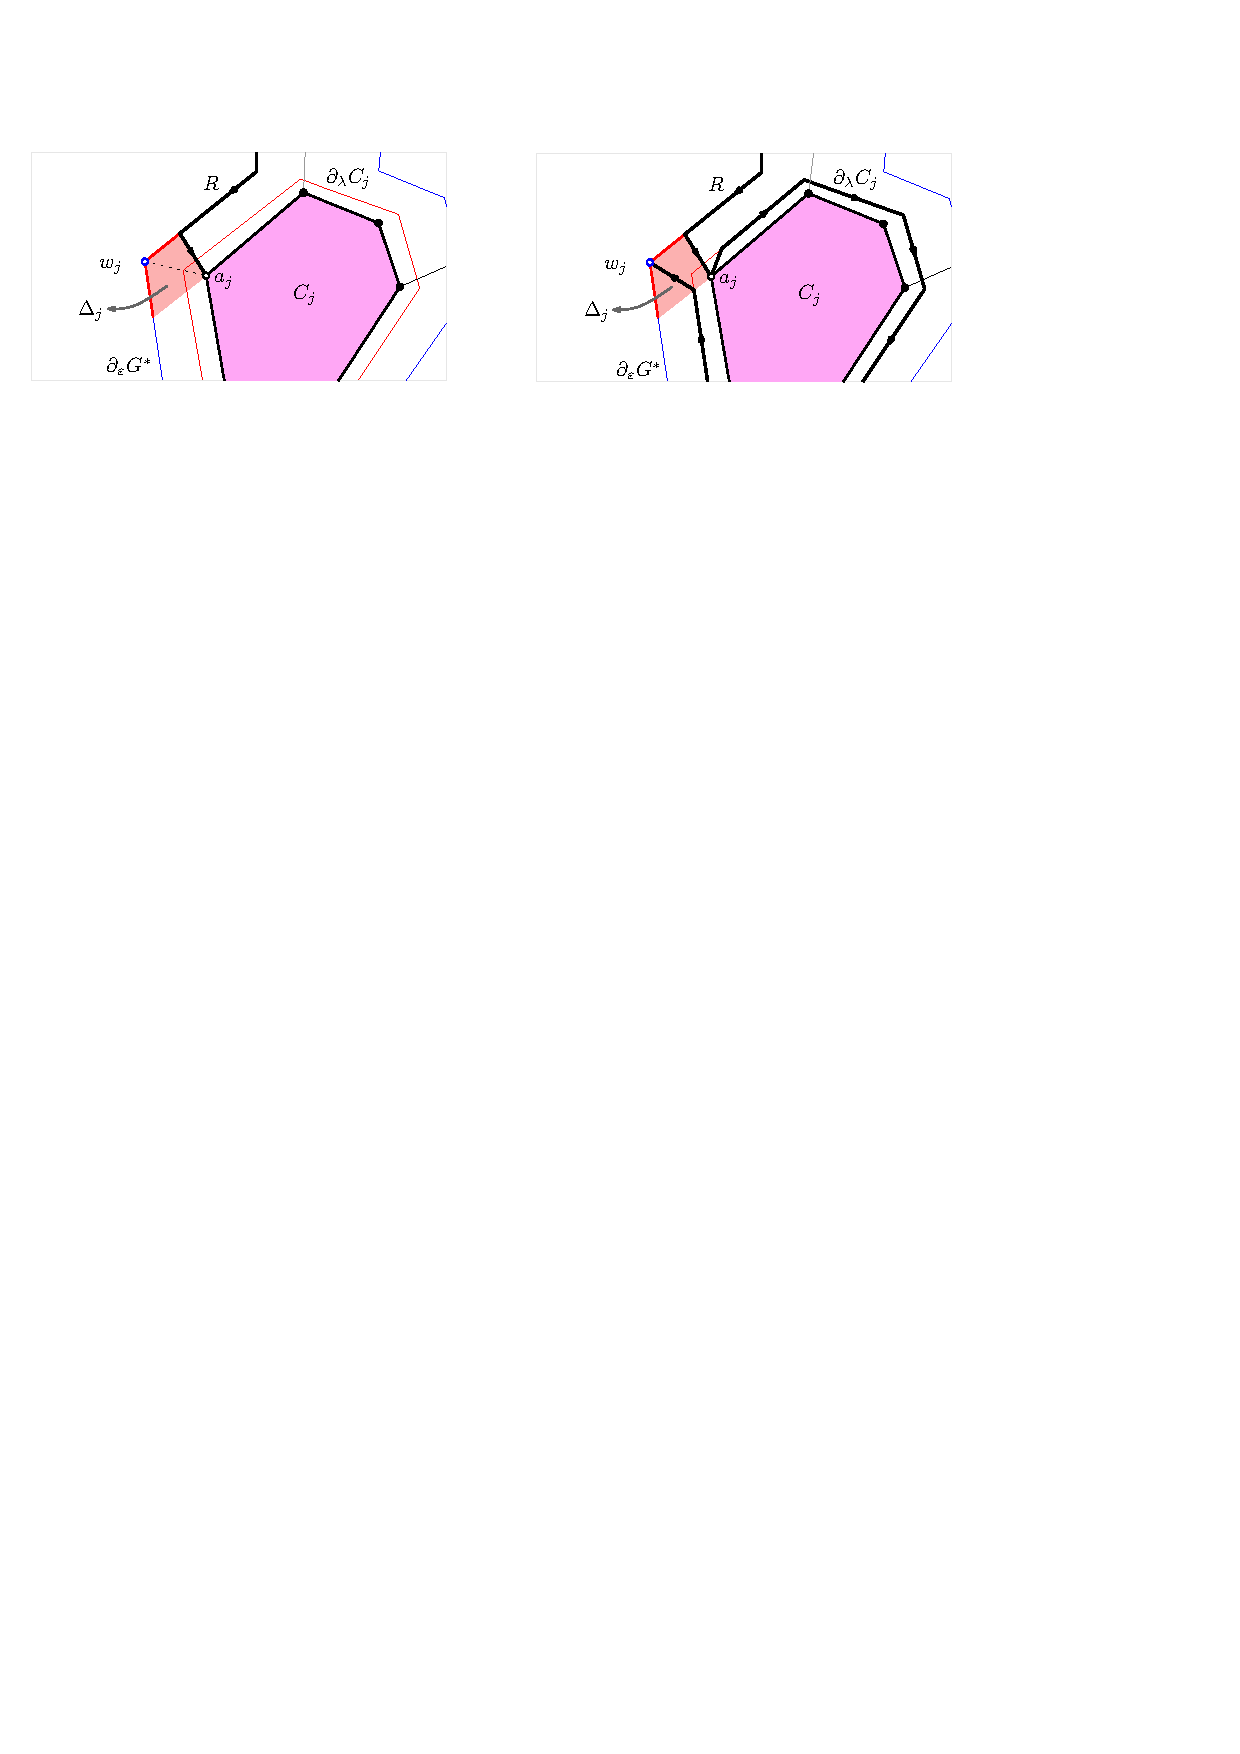
\includegraphics{img/ComponentToTheRight.pdf}
\caption{\small When extending $R$ from $a_j$ to $a_{j+1}$ we keep $C_j$ to the right of $R$.}
\label{fig: Component to the right}
\end{figure}

The path from $a_j$ to $a_{j+1}$ continues with a path from $w_j$ to $w_{j+1}$, which follows the unique path in $\partial_\varepsilon G^*$ from $w_j$ to $w_{j+1}$. However, whenever we reach an endpoint of $N_i$ for some $i\in \{1,\dots,r\}$ such that $i>j+1$, we take a detour to the other endpoint of $N_i$ while avoiding its interior so that the points in the interior of $N_i$ remain $R$-visible from $a_i$; see Figure~\ref{fig:Skip Component}. Formally, we walk from the reached endpoint of $N_i$ to $\partial_\delta C_i\setminus \Delta_i$ along the boundary of $\Delta_i$. Then, we traverse the path $\partial_\delta C_i\setminus \Delta_i$ before moving to the other endpoint of $N_i$ from the endpoint of $\partial_\delta C_i \setminus \Delta_i$. In this way, we avoid crossing the cone $\Delta_i$. Note that $R$ does not intersect the interior of the simple polygon bounded by $\partial_\delta C_i$ nor the interior of $\Delta_i$. Moreover, $R$ remains inside the simple polygon bounded by $\partial_\varepsilon G^*$.

\begin{figure}[b]
\centering
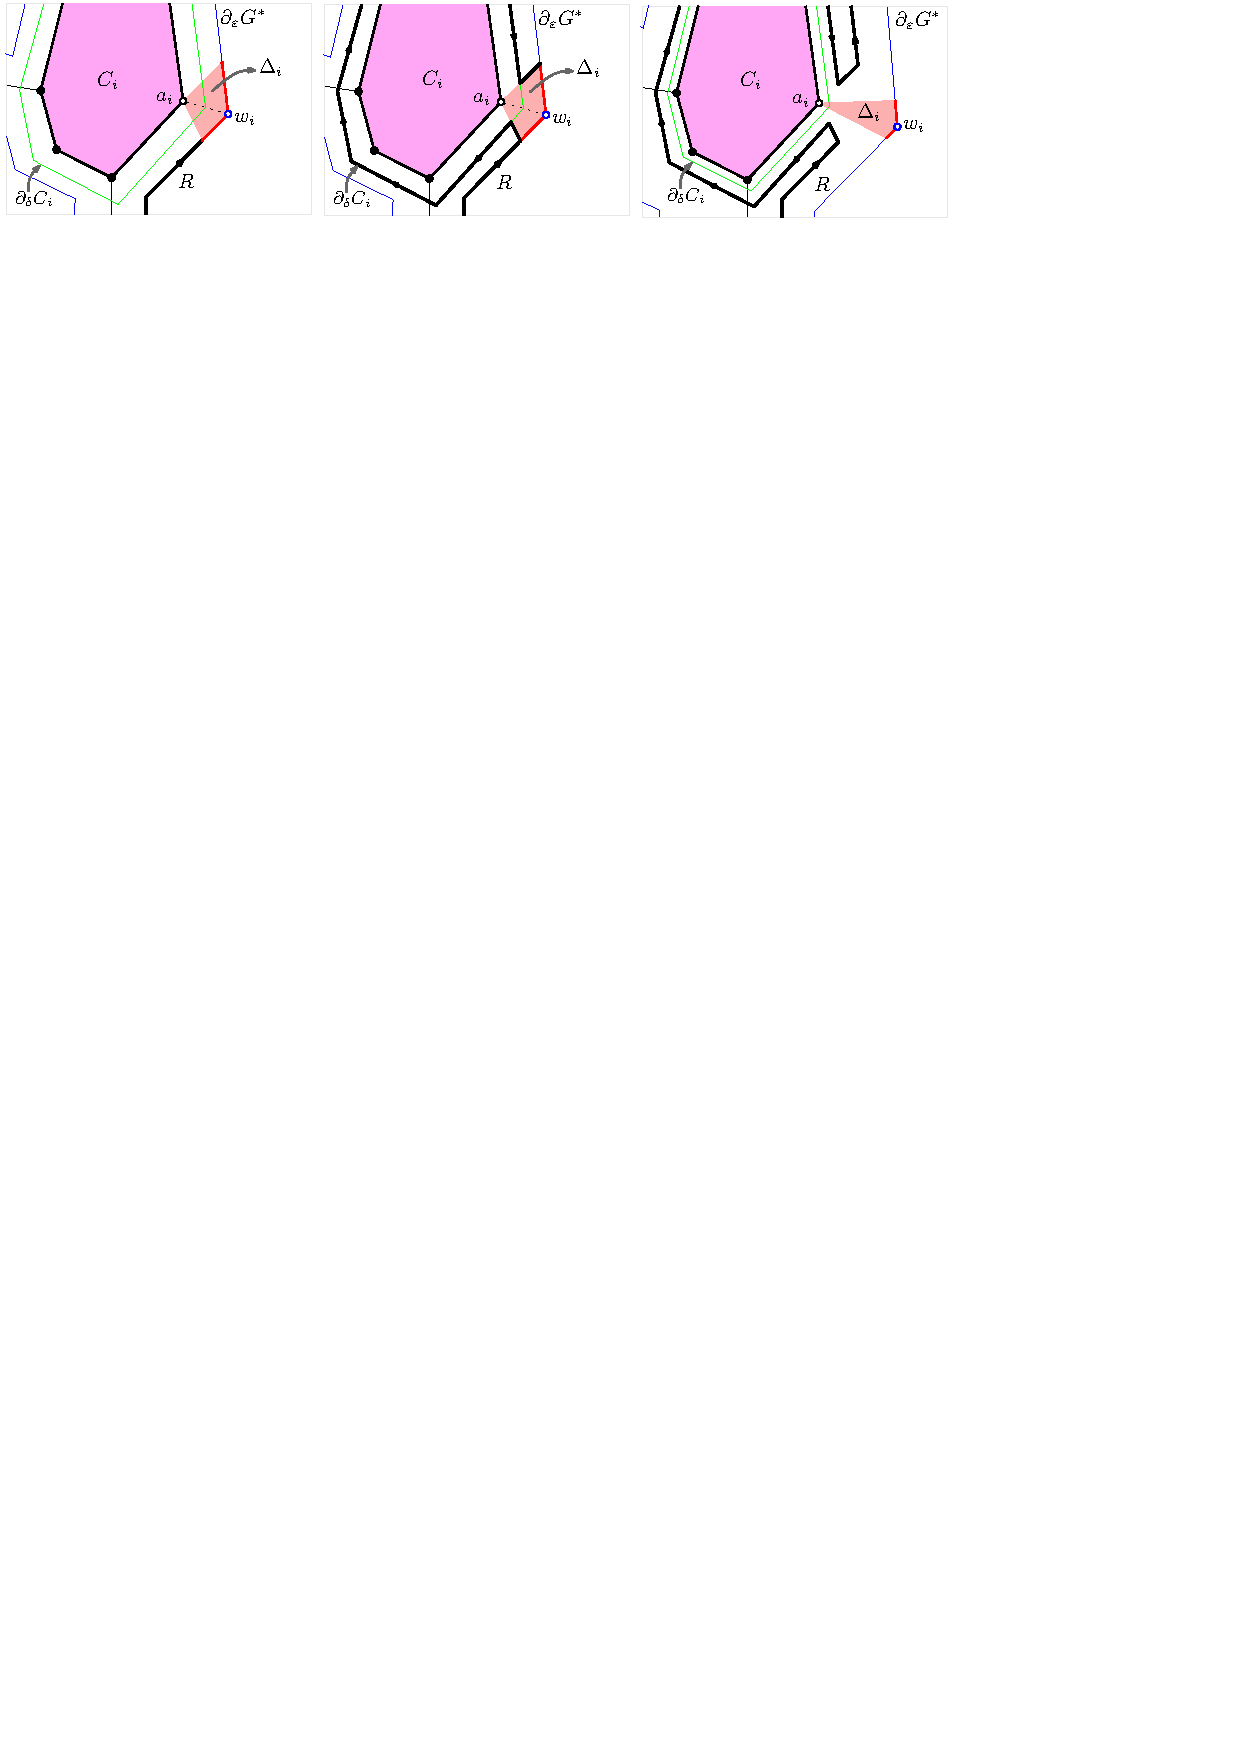
\includegraphics{img/SkipComponent.pdf}
\caption{\small The ``detour'' taken to avoid crossing the cone $\Delta_i$ (left, middle); and the narrowing of the cone $\Delta_i$ as well as the redefinition of the $\varepsilon$- and $\delta$-fattenings of $G^*$ and $C_i$, respectively.}
\label{fig:Skip Component}
\end{figure}

Once we go around $C_i$, we are back on $\partial_\varepsilon G^*$ on the other endpoint of $N_i$. In this way, we continue going towards~$w_{j+1}$ along $\partial_\varepsilon G^*$ until reaching an endpoint of $N_{j+1}$.
Once we reach an endpoint of $N_{j+1}$, we move directly from this endpoint to $a_{j+1}$.

Because $\partial_\varepsilon G^*$ is isomorphic to $\varphi$, the constructed path between $a_j$ and $a_{j+1}$ has length at most $|\varphi(a_j, a_{j+1})|$ plus the length of the boundaries of the components that we walked around. Because each component we walked around has its attachment corner on the path $\varphi(a_j, a_{j+1})$, and thus in $A(a_j, a_{j+1})$, the length of the constructed path between $a_j$ and $a_{j+1}$ is
\[ O\left(|\varphi(a_j, a_{j+1})| + \sum_{a_i\in A(a_j, a_{j+1})} |C_i|\right) = O(\sigma_G(a_j, a_{j+1})) \enspace .
\]

After reaching $a_{j+1}$, we increase $\varepsilon$ by a factor of two. Similarly, we decrease the value of $\delta$ by a factor of two. That is, after reaching $a_{j+1}$, $\varepsilon = \mu 2^{j+1}$ while $\delta = \mu/2^{j+1}$ and hence, we guarantee that $\lambda < \delta < \varepsilon$.
Also, $\partial_\varepsilon G^*$ is still simple, provided that $\mu$ is initially chosen to be sufficiently small.
Finally, we reduce $\tau$ by a factor of two and update $N_i$ and $\Delta_i$ accordingly, for each $i\in \{1,\dots,n\}$; see Figure~\ref{fig:Skip Component} (right).

Recall that for each $a_i\notin R$, $R$ intersected neither the interior of $\Delta_i$ nor the interior of the polygon bounded by $\partial_\delta C_i$. Moreover, $R$ remained within $\partial_\varepsilon G^*$.
Therefore, after increasing (\emph{resp.} reducing) $\varepsilon$ (\emph{resp.} $\delta$), we preserve the escape invariant for the next iteration of the algorithm.
We iterate until all attachment corners of $G$ are visited by $R$.

\begin{lemma}\label{lemma:Path for connected augmentations} \appendixproof
Given an arbitrary order $a_1, \ldots, a_r$ of the attachment corners of $G$, there is a path $R$ connecting all attachment corners of $G$ in the given order such that $R\cup G$ is planar, every component $C_i$ of $G$ lies to the right of $R$ when oriented from $a_1$~to~$a_r$, and the subpath of $R$ between $a_j$ and $a_{j+1}$ has $O(\sigma_G(a_j, a_{j+1}))$ vertices, for each $j\in \{1,\dots,r-1\}$.
\end{lemma}

Figure~\ref{figure:big-example} illustrates the preceding algorithm on a small example.  In this example, the path from $a_1$ to $a_2$ passes by $a_4$, so $R$ detours around $C_4$ in order to preserve the escape invariant at $a_4$.  After $R$ attaches to $a_2$ and $a_3$, it winds around components $C_2$ and $C_3$, respectively, in order to ensure that these components attach to the right of $R$.


\subsection{Compatible drawings of planar graphs}
Let $\mathcal G$ be a planar graph with $n$ vertices and $r$ connected
components.  Let $G_1, \ldots, G_k$ be $k$ planar isomorphic drawings
of $\mathcal G$.  For now, we will assume that, in these drawings,
every component of $\mathcal G$ has at least one vertex incident to
the outer face.  (In the Appendix, we show that this is not a real
restriction; one can apply the same algorithm to each face of $\mathcal
G$.)  We show how to construct a compatible augmentation of $\mathcal G$
of size $O(nr^{1-1/k})$.

Let $\mathcal C_1, \ldots, \mathcal C_r$ be the connected components of $\mathcal G$.  Because $G_1,\ldots,G_k$ are isomorphic, we can select one attachment corner from each component in the drawing $G_1$, and this attachment corner also appears in each of $G_2,\ldots,G_k$. Thus, for each $j\in\{1,\ldots,r\}$, we choose an attachment corner $a_j$ of $\partial C_j$ such that $a_j$ is incident to the outer face of $C_j$.

\begin{figure}
   \centering{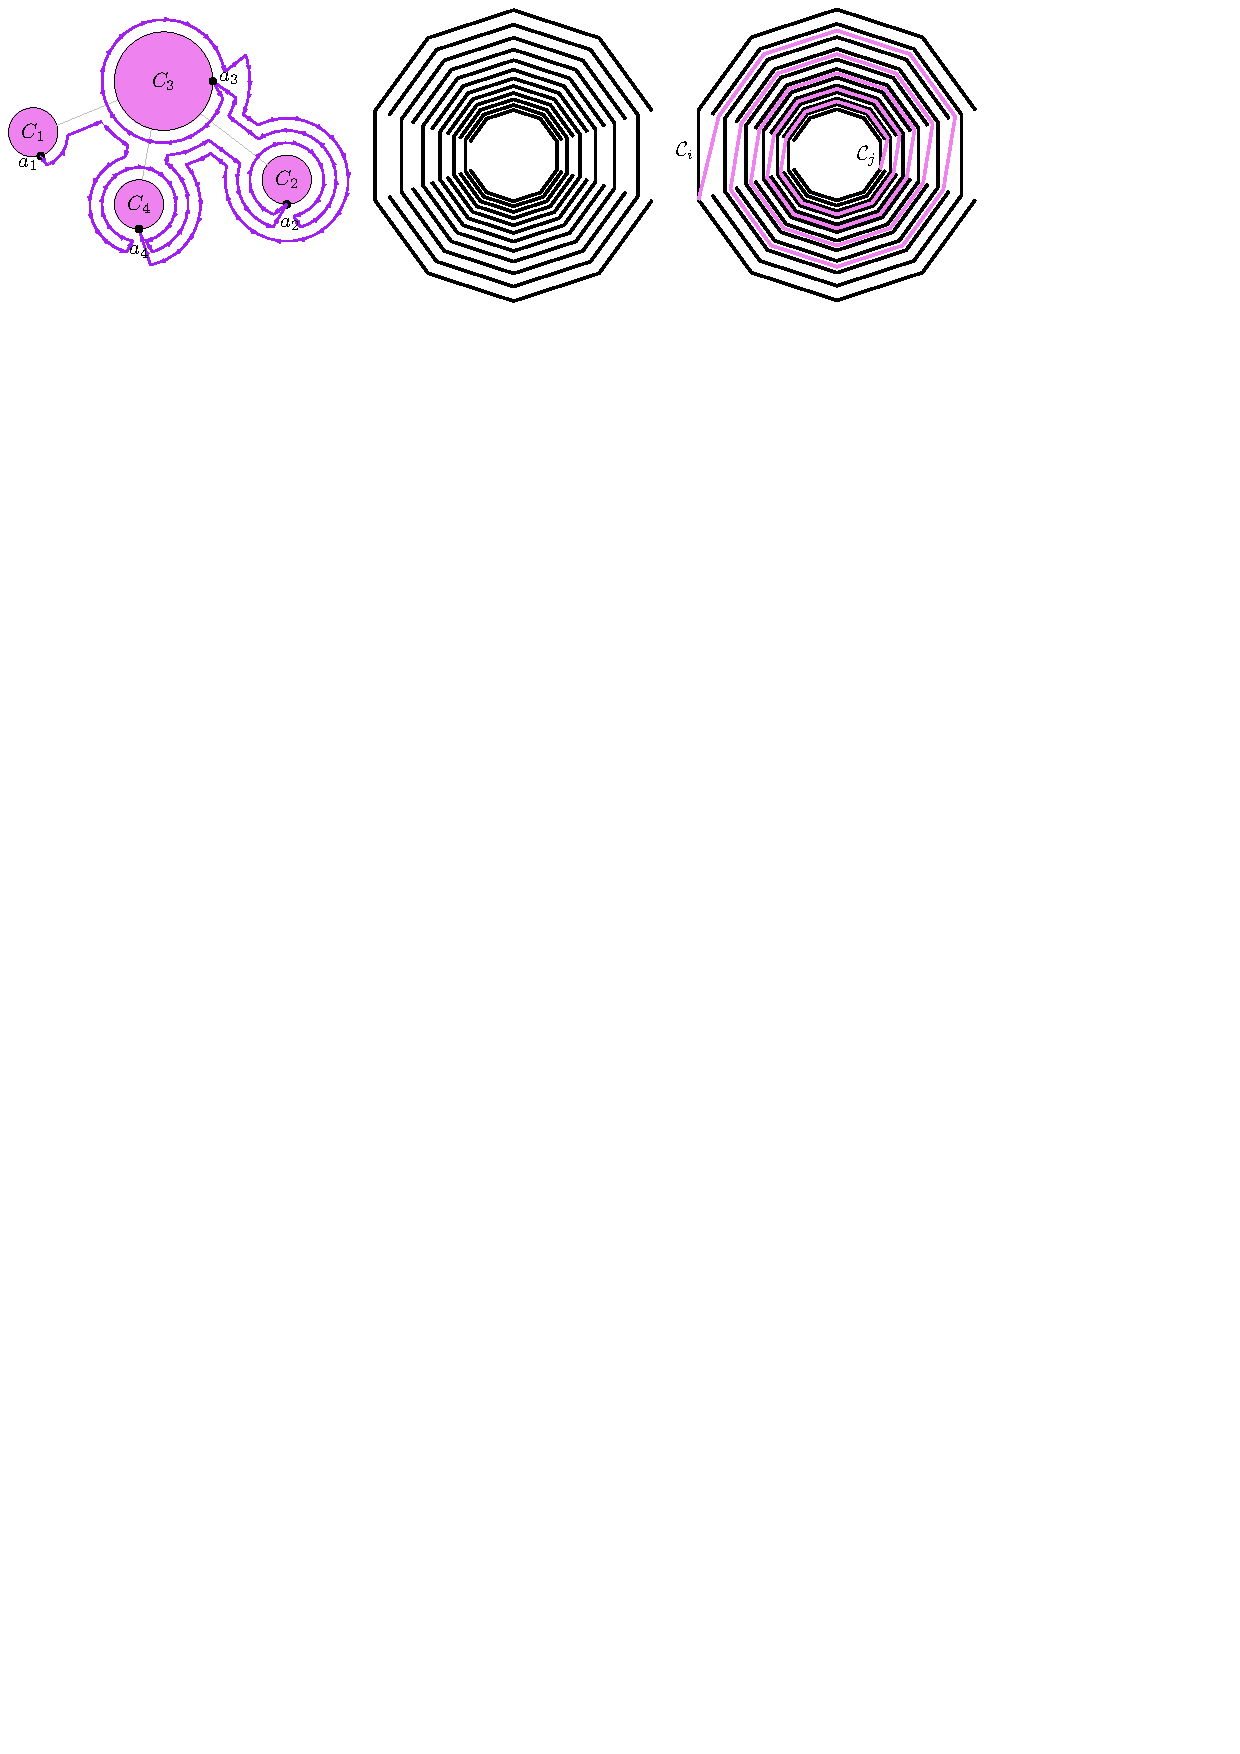
\includegraphics{img/big-example}}
   \caption{\small An example of the algorithm for generating a spanning path that connects $a_1,\ldots,a_4$.}
   \label{figure:big-example}
\end{figure}

For each $i\in \{1,\dots,k\}$, let $G_i^*$ be a connected augmentation of $G_i$, as defined in Section~\ref{section: connected augmentations}. For each $i\in\{1,\ldots,k\}$ and $j\in\{1,\ldots,r\}$, let $\rank_i(j) = \sigma_{G_i}(a_1, a_j)$. For each $j\in\{1,\ldots,r\}$, let $x_j\in \mathbb{R}^k$ be a point corresponding to the component $C_j$ such that $x_j = (\rank_1(a_j), \rank_2(a_j), \ldots, \rank_k(a_j))$. Let $X = \{x_1, \ldots, x_r\}\subset\R^k$ denote the resulting set of points. Lemma~\ref{lemma:Contained in integer grid} implies that $X$ is contained in an integer grid of side length $4n$.

Let $P$ be the shortest $\ell_\infty$ Hamiltonian path of $X$. Because $X$ is contained in the $k$-dimensional box of side-length $4n$ and $|X| = r$, the maximum ($\ell_\infty$) length of $P$ is $O(nr^{1-1/k})$~\cite{few:shortest}. Note that the order of the points in $P$ induces an order of the components of $\mathcal G$ and hence an order of the attachment corners of each $G_i$.

\begin{theorem}\label{theorem:main}
For each $1\leq i\leq k$, we can construct a path $R_i$ of length $O(nr^{1-1/k})$ that connects every component of $G_i$ such that $G_i\cup R_i$ is planar. Moreover, for each $1\leq i<j\leq k$, $G_i\cup R_i$ is isomorphic to $G_j\cup R_j$.
\end{theorem}
\begin{proof}
By relabelling, let $(a_1, \ldots, a_r)$ denote the order of the attachment corners of $G_i$ induced by $P$.  Letting $d_j$ denote the $\ell_\infty$ distance between $x_j$ and $x_{j+1}$, we denote by $\mathcal{H}$ a path that passes through (the vertices corresponding to corners) $a_1, \ldots, a_r$ in this order, and that includes an additional $O(d_j)$ vertices between $a_{j}$ and $a_{j+1}$.  Thus, the number of vertices in $\mathcal{H}$ is proportional to the length of $P$, which is $O(nr^{1-1/k})$.

For each $G_i$, we use Lemma~\ref{lemma:Path for connected augmentations} to draw $\mathcal{H}$ as a planar path, $R_i$, that connects $a_1, \ldots, a_r$ in this order. Since $|\rank_i(j+1) - \rank_i(j)|$ represents the difference in the $i$-th coordinates of $x_j$ and $x_{j+1}$, by the triangle inequality we infer that $|\rank_i(j+1) - \rank_i(j)| \leq  d_j$. Thus, the $O(d_j)$ vertices in $\mathcal{H}$ between $a_j$ and $a_{j+1}$ are enough to
draw the $O(|\rank_i(j+1) - \rank_i(j)|)$ vertices in $R_i$ between $a_j$ and $a_{j+1}$. 

% For each $G_i$, we use Lemma~\ref{lemma:Path for connected augmentations} to construct a plane path $R_i$ that connects the attachment corners of $G_i$ in the order induced by $P$. Assume that $(a_1, \ldots, a_r)$ is the order of the attachment corners of $G_i$ induced by $P$. Lemma~\ref{lemma:Path for connected augmentations} implies that $|R_i| = O(\sum_{j=1}^{n-1} \sigma_{G_i}(a_j, a_{j+1}))$.

%Because $\sigma_{G_i}(a_j, a_{j+1}) = |\sigma_{G_i}(a_1, a_{j+1}) - \sigma_{G_i}(a_1, a_j)|$ by Lemma~\ref{lemma:Contained in integer grid} and since $\rank_i(j) = \sigma_{G_i}(a_1, a_j)$, we get that  $\sigma_{G_i}(a_j, a_{j+1}) = |\rank_i(j+1) - \rank_i(j)|$. Therefore, $|R_i|  = O\left(\sum_{j=1}^{n-1} |\rank_i(j+1) - \rank_i(j)|\right)$.

% Let $d_j$ denote the distance between $x_j$ and $x_{j+1}$ in $P$. Because $|\rank_i(j+1) - \rank_i(j)|$ represents the difference in the $i$-th coordinates of $x_j$ and $x_{j+1}$, by the triangle inequality we infer that $|\rank_i(j+1) - \rank_i(j)| \leq  d_j$ . Thus, the path $R_i$ has length $O\left(\sum_{j=1}^{n-1} |\rank_i(j+1) - \rank_i(j)|\right) = O(\sum_{j=1}^{n-1} d_j)$. Because $\sum_{j=1}^{n-1} d_j = |P| = O(nr^{1-1/k})$, the length $R_i$ is $O(nr^{1-1/k})$.

To conclude, each $R_i$ visits each component only at its attachment corner, the attachment corners of each $G_i$ are connected in the same order, and $R_i$ leaves every component to the right when oriented from $a_1$ to $a_r$. Therefore, $G_i\cup R_i$ is isomorphic to $G_j\cup R_j$ for each $1\leq i<j\leq k$.
\end{proof}


The construction in Theorem~\ref{theorem:main} is implemented fairly easily using existing algorithmic tools, including plane-sweep and minimum spanning trees, yielding an algorithmic version:

\begin{theorem}
  An augmentation satisfying the conditions of Theorem~\ref{theorem:main}
  can be computed in $O(kn^2)$ time for any value of $k$.  If $k$ is
  constant, then the augmentation can be computed in $O(nr^{1-1/k})$
  time.
\end{theorem}



\section{Lower Bounds}\label{section:Lower bound}
%\vspace{-.1in}
Our lower bounds are based on the following lemma. It says that we can find $k$ permutations of $\{1,\ldots,r\}$ such that for half the indices $i\in\{1,\ldots,r\}$, and every $j\in\{1,\ldots,r\}\setminus\{i\}$, there is a permutation in which $i$ and $j$ are at distance $\Omega(r^{1-1/k})$.

\begin{lemma}\label{lem:permutations}\appendixproof
For $k>1$ and $1\leq r\leq n$, let $t=(1/2)^{1+1/k}\cdot(r-1)^{1-1/k}$.  There exists permutations $\pi^{(1)},\ldots,\pi^{(k)}$ of $\{1,\ldots,r\}$ such that for at least half the values of $i\in\{1,\ldots,r\}$ and for every $j\in\{1,\ldots,r\}\setminus\{i\}$,
\begin{equation}
 \max\left\{\left|\pi^{(s)}_i-\pi^{(s)}_j\right|\colon s\in\{1,\ldots,k\} \right\}
 \ge t \enspace .
     \label{eq:perm}
\end{equation}
\end{lemma}

Using Lemma~\ref{lem:permutations}, we can prove a lower bound that matches the upper bound obtained in our general construction.

\begin{theorem}\label{thm:lower-bound}
  For every positive integer $n$, every $r\in\{2,\ldots,\lfloor
  n/4\rfloor\}$, and every integer $k>1$, there exists a graph $\mathcal
  G$ having $n$ vertices, $1\leq r\leq n$ connected components, and
  $k$ isomorphic drawings $G_1,\ldots,G_k$ such that any compatible
  augmentation of $\mathcal G$ has size $\Omega(nr^{1-1/k})$.
\end{theorem}

\begin{proof}
Since the lemma only claims an asymptotic result, we may assume without
loss of generality that $r$ is even and that $2r$ divides $n$.

The graph $\mathcal G$ consists of $r$ disjoint paths,
$\mathcal{C}_1,\ldots,\mathcal{C}_r$, each of length $n/r$.  Each of the
drawings $G_1$,\ldots,$G_k$ draws the vertices of $\mathcal G$ on the
same point and edge set. The point set consists of the vertices of
$r$ nested regular $n/r$-gons, $P_1,\ldots,P_r$, each centered at the
origin and having nearly the same size. Refer to Figure~\ref{figure:lower-bound}. More precisely, $P_1\subset P_2\subset\cdots\subset P_r$ and the sizes are chosen so that any segment
joining two non-consecutive vertices of $P_i$ intersects the interior
of~$P_{i-1}$.
The drawings $G_1,\ldots,G_k$ are obtained from the permutations
$\pi^{(1)},\ldots,\pi^{(k)}$ given by \linebreak Lemma~\ref{lem:permutations}.
In the drawing $G_x$, the path $\mathcal C_i$ is drawn on the vertices
of $P_{\pi^{(x)}_i}$. If $y=\pi^{(x)}_i$ is even, the drawing uses
all the edges of $P_y$ except the left-most edge.  If $y$ is odd, the
drawing uses all the edges of $P_y$ except the right-most edge.

\begin{figure}
  \centering{
    \begin{tabular}{c@{\hspace{1cm}}c}
      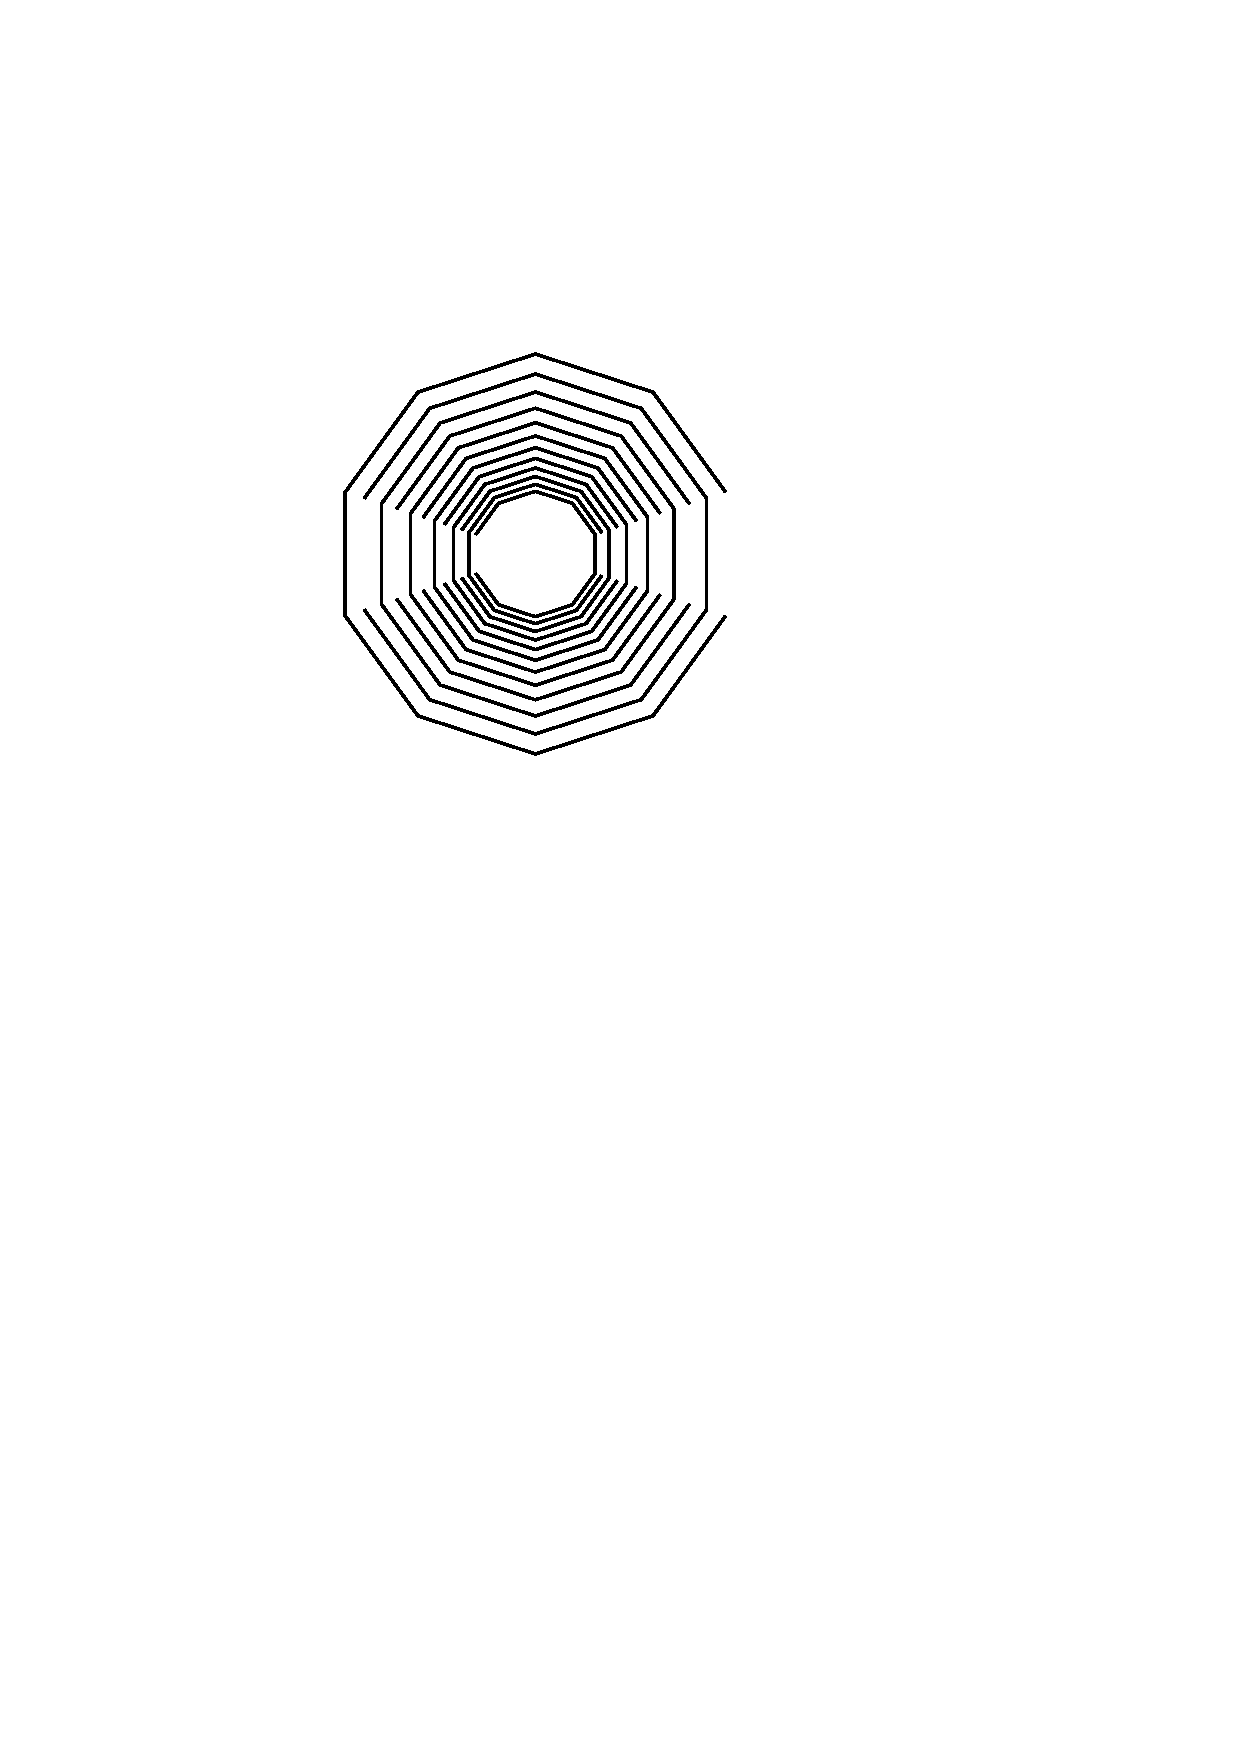
\includegraphics[scale=0.75]{img/lower-bound-1} & 
      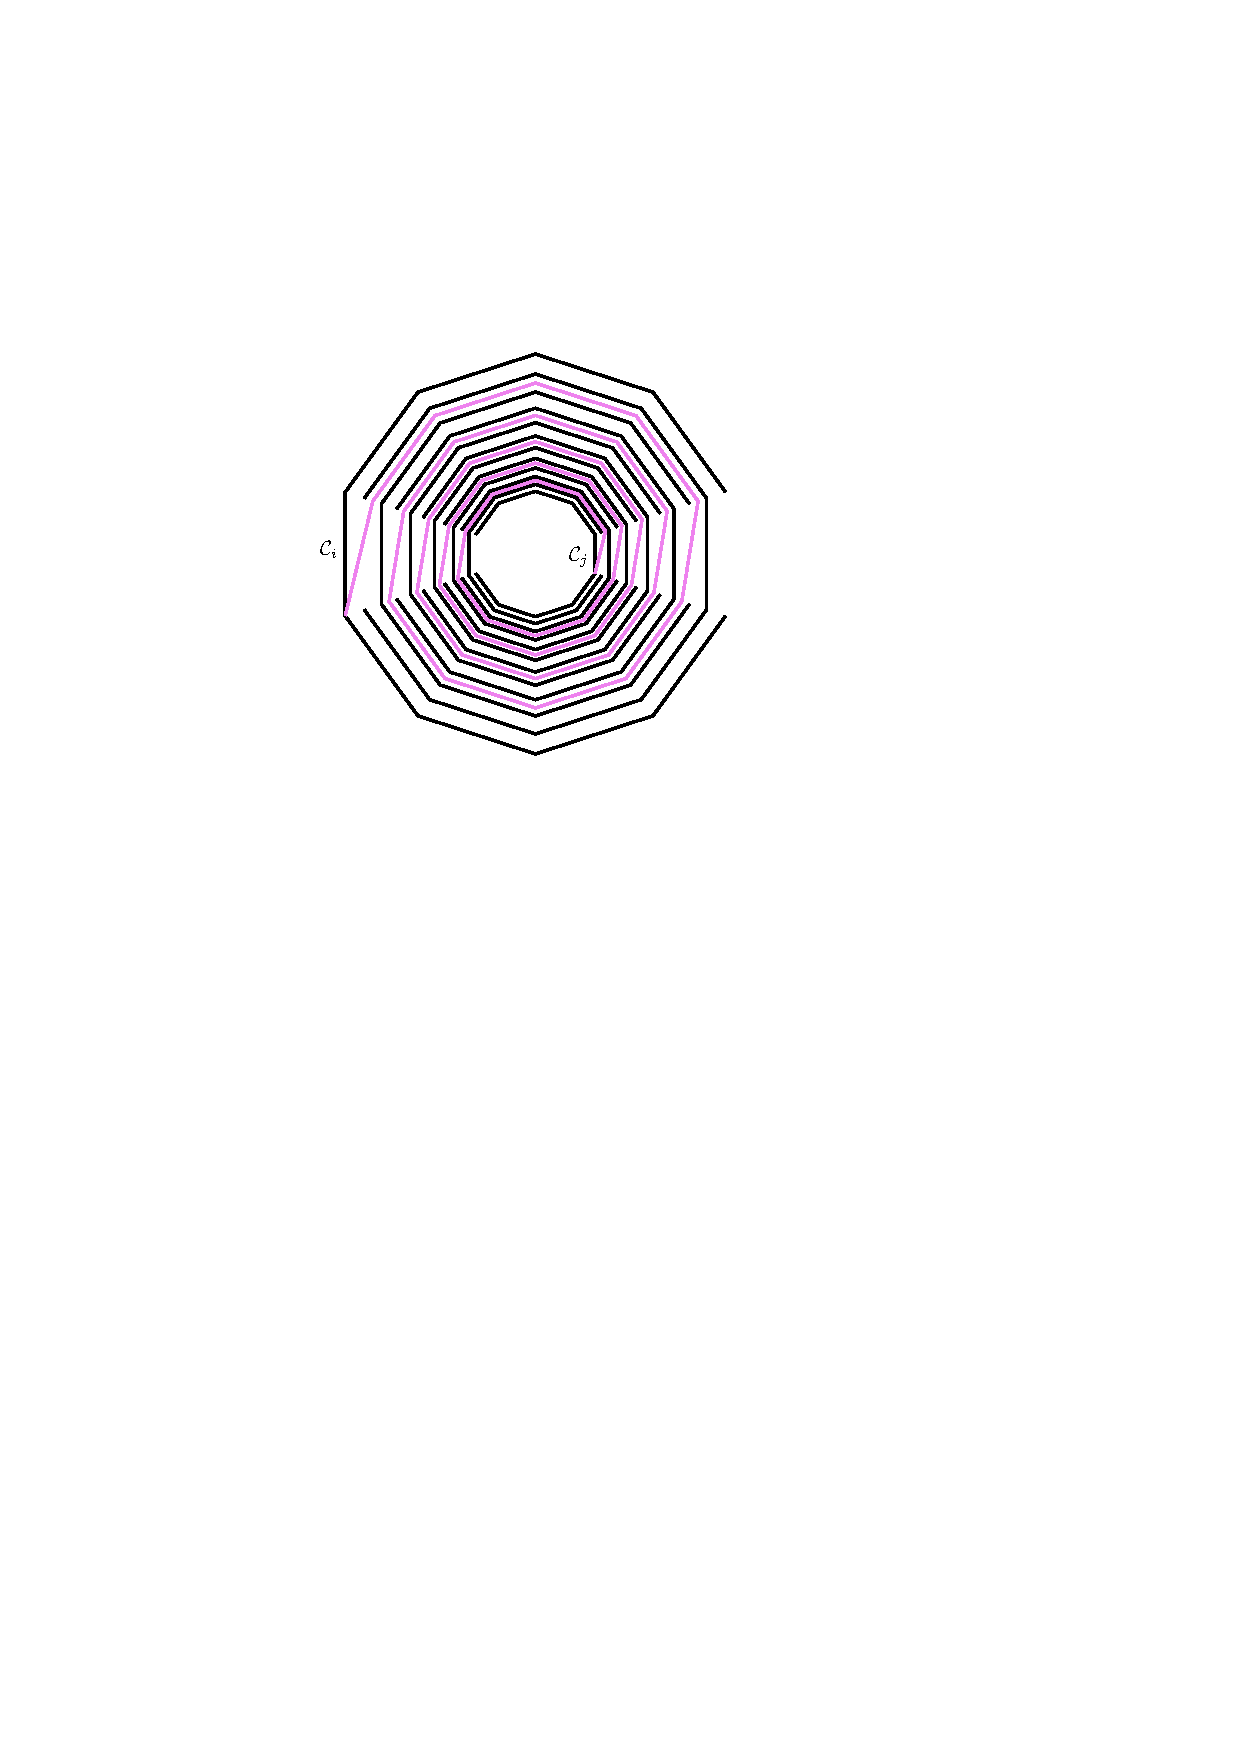
\includegraphics[scale=0.75]{img/lower-bound-2}
    \end{tabular}
  }
  \caption{In the construction in Theorem~\ref{thm:lower-bound}, all drawings use the same set of vertices and line segments and the drawing of a path that joins $\mathcal C_i$ to $\mathcal C_j$ must travel around all paths drawn between the drawing of $\mathcal C_i$ and $\mathcal C_j$.}
  \label{figure:lower-bound}
\end{figure}


Now, without loss of generality, consider some edge-minimal compatible
augmentation $\mathcal H$ of $\mathcal G$.  For each component
$\mathcal{C}_i$ of $G$, let $T_i$ be any path in $\mathcal H$ that has
one endpoint on $\mathcal C_i$, one endpoint on some other component
$\mathcal{C}_j$, $j\neq i$, and no vertices of $\mathcal G$ in its
interior.
Now, for each of the $r/2$ indices $i\in\{1,\ldots,r\}$ that satisfy
\eqref{eq:perm}, the path $T_i$ joins a vertex of
$P_{\pi^{(s)}_i}$ to a vertex of $P_{\pi^{(s)}_j}$, $j\neq
i$, and $|\pi^{(s)}_i-\pi^{(s)}_i|\ge t$.  This path must
have length $\Omega(tn/r)$ since it has to ``go around'' the
paths between $P_{\pi^{(s)}_i}$ and $P_{\pi^{(s)}_j}$; see
Figure~\ref{figure:lower-bound} (right).

Thus far, we have shown that for at least $r/2$ values of
$i\in\{1,\ldots,r\}$, the component $C_i$ is the endpoint of a
path, $T_i$, of length at least $\Omega(tn/r)=\Omega(nr^{-1/k})$.
It is tempting to claim the result at this point, since
$(r/2)\cdot\Omega(nr^{-1/k})=\Omega(nr^{1-1/k})$. Unfortunately, there
is a little more work that needs to be done, since two such paths $T_i$
and $T_j$ may not be disjoint, so summing their lengths double-counts
the contribution of the shared portion.

To finish up we note that, since the augmentation $\mathcal{H}$ is minimal,
it is a tree; $\mathcal G$ contains no cycles, so any cycle in $\mathcal H$ contains an edge not in $\mathcal G$ that could be removed.  Now, observe that if we traverse the outer face of (any planar drawing of) $\mathcal H$ then we obtain a non-simple path, $P$, that traverses each edge of $\mathcal{H}$ exactly twice. If we consider the set of maximal subpaths of $P$ with no vertex of $\mathcal G$ in their interior, we obtain a set of $r$ paths, $Q_1,\ldots,Q_{r}$ and, for every component $\mathcal C_i$ of $\mathcal G$, there is a vertex of $\mathcal C_i$ that is an endpoint of at least one such path.  Therefore, from the preceding discussion, the total length of $Q_1\ldots,Q_{r}$ is $\Omega(nr^{1-1/k})$.  But since each edge of $\mathcal H$ appears at most twice in these subpaths, we conclude that $\mathcal H$ has $\Omega(nr^{1-1/k})$ edges.  Since $\mathcal H$ is a tree, it has $\Omega(nr^{1-1/k})$ vertices.
\end{proof}

\newpage

\section*{Acknowledgement}
This work was initiated at the \emph{Second Workshop on Geometry and Graphs},
held at the Bellairs Research Institute, March 9-14, 2014.  We are
grateful to the other workshop participants for providing a stimulating
research environment.

% \section{Summary and Conclusions}\label{section:Conclusions}
% I have nothing to write here.  Some open problems might be nice.
\bibliographystyle{plain}
\bibliography{CompatibleEmbeddings}















\end{document}
